\documentclass[10pt]{beamer}

\usecolortheme{default}

\setbeamertemplate{footline}[page number]{}
\setbeamertemplate{frametitle}[default][left]
\setbeamerfont{title}{size=\Large}
% \usetheme{Singapore} %{Warsaw}{Darmstadt}
\beamertemplatenavigationsymbolsempty

\setbeamersize{text margin left=3mm,text margin right=3mm} 

% отображать название слайда слева

% load packages
\usepackage[utf8]{inputenc}
\usepackage[russian]{babel}
\usepackage{graphicx, epsfig}
\usepackage{subfig}
\usepackage{floatflt}
\usepackage{epic,ecltree}
\usepackage{mathtext}
\usepackage{fancybox}
\usepackage{fancyhdr}
\usepackage{multirow}
\usepackage{enumerate}
\usepackage{epstopdf}
\usepackage{multicol}
\usepackage{algorithm}
\usepackage[noend]{algorithmic}
\usepackage{amsmath,amsfonts,amssymb,amsthm,mathtools} % AMS

\def\algorithmicrequire{\textbf{Input:}}
\def\algorithmicensure{\textbf{Output:}}

% latin bold lower
\newcommand{\ba}{\mathbf{a}} 
\newcommand{\bb}{\mathbf{b}}
\newcommand{\bc}{\mathbf{c}} 
\newcommand{\be}{\mathbf{e}} 
\newcommand{\bh}{\mathbf{h}} 
\newcommand{\bp}{\mathbf{p}} 
\newcommand{\bq}{\mathbf{q}}
\newcommand{\bt}{\mathbf{t}} 
\newcommand{\bs}{\mathbf{s}} 
\newcommand{\bu}{\mathbf{u}} 
\newcommand{\bv}{\mathbf{v}} 
\newcommand{\bw}{\mathbf{w}} 
\newcommand{\bx}{\mathbf{x}} 
\newcommand{\by}{\mathbf{y}} 
\newcommand{\bz}{\mathbf{z}} 

% latin bold upper
\newcommand{\bA}{\mathbf{A}} 
\newcommand{\bB}{\mathbf{B}} 
\newcommand{\bC}{\mathbf{C}} 
\newcommand{\bD}{\mathbf{D}} 
\newcommand{\bE}{\mathbf{E}}
\newcommand{\bF}{\mathbf{F}}
\newcommand{\bH}{\mathbf{H}}
\newcommand{\bI}{\mathbf{I}} 
\newcommand{\bJ}{\mathbf{J}}
\newcommand{\bM}{\mathbf{M}} 
\newcommand{\bP}{\mathbf{P}}
\newcommand{\bQ}{\mathbf{Q}}
\newcommand{\bR}{\mathbf{R}}
\newcommand{\bS}{\mathbf{S}}
\newcommand{\bT}{\mathbf{T}} 
\newcommand{\bU}{\mathbf{U}} 
\newcommand{\bV}{\mathbf{V}} 
\newcommand{\bW}{\mathbf{W}} 
\newcommand{\bX}{\mathbf{X}} 
\newcommand{\bY}{\mathbf{Y}} 
\newcommand{\bZ}{\mathbf{Z}} 

% latin cal upper
\newcommand{\cA}{\mathcal{A}}
\newcommand{\cD}{\mathcal{D}}
\newcommand{\cL}{\mathcal{L}} 
\newcommand{\cN}{\mathcal{N}} 
\newcommand{\cS}{\mathcal{S}} 
\newcommand{\cT}{\mathcal{T}} 
\newcommand{\cW}{\mathcal{W}} 
\newcommand{\cX}{\mathcal{X}} 
\newcommand{\cZ}{\mathcal{Z}} 

% latin bb upper
\newcommand{\bbE}{\mathbb{E}} 
\newcommand{\bbP}{\mathbb{P}} 
\newcommand{\bbR}{\mathbb{R}} 
\newcommand{\bbT}{\mathbb{T}}
\newcommand{\bbU}{\mathbb{U}}
\newcommand{\bbX}{\mathbb{X}}
\newcommand{\bbY}{\mathbb{Y}}
\newcommand{\bbZ}{\mathbb{Z}}

% greek bold lower
\newcommand{\bepsilon}{\boldsymbol{\varepsilon}}
\newcommand{\btheta}{\boldsymbol{\theta}} 
\newcommand{\blambda}{\boldsymbol{\lambda}} 
\newcommand{\bchi}{\boldsymbol{\chi}}
\newcommand{\bnu}{\boldsymbol{\nu}}
\newcommand{\bpi}{\boldsymbol{\pi}} 
\newcommand{\bmu}{\boldsymbol{\mu}} 
\newcommand{\btau}{\boldsymbol{\tau}}
\newcommand{\bsigma}{\boldsymbol{\sigma}} 
\newcommand{\bupsilon}{\boldsymbol{\upsilon}}
\newcommand{\bphi}{\boldsymbol{\phi}} 
\newcommand{\bpsi}{\boldsymbol{\psi}} 

% greek bold upper
\newcommand{\bSigma}{\boldsymbol{\Sigma}} 
\newcommand{\bTheta}{\boldsymbol{\Theta}}

% min/max
\newcommand{\argmin}{\mathop{\arg \min}\limits}
\newcommand{\argmax}{\mathop{\arg \max}\limits}

% transpose
\newcommand{\T}{^{\text{\tiny\sffamily\upshape\mdseries T}}}

% zero one matrices
\newcommand{\bOne}{\boldsymbol{1}}
\newcommand{\bZero}{\boldsymbol{0}}

% russian style 
\renewcommand{\epsilon}{\ensuremath{\varepsilon}}
\renewcommand{\phi}{\ensuremath{\varphi}}
\renewcommand{\kappa}{\ensuremath{\varkappa}}
\renewcommand{\le}{\ensuremath{\leqslant}}
\renewcommand{\leq}{\ensuremath{\leqslant}}
\renewcommand{\ge}{\ensuremath{\geqslant}}
\renewcommand{\geq}{\ensuremath{\geqslant}}
\renewcommand{\emptyset}{\varnothing}

\newcommand\undermat[2]{%f
	\makebox[0pt][l]{$\smash{\underbrace{\phantom{%
					\begin{matrix}#2\end{matrix}}}_{\text{$#1$}}}$}#2}

\newtheorem{statement}{Утверждение}
\newtheorem{rustheorem}{Теорема}

%%% Рисунки
\usepackage{tikz}
\usetikzlibrary{matrix}

%\definecolor{beamer@blendedblue}{RGB}{15,120,80}
%----------------------------------------------------------------------------------------------------------
\title[\hbox to 56mm{  \hfill\insertframenumber\,/\,\inserttotalframenumber}]
{\\ Снижение размерности пространства \\ в задачах декодирования сигналов}
\author[Роман Исаченко]{\\ 
	Исаченко Роман Владимирович \\
	\vspace{3mm}
	{\footnotesize 
	Диссертация на соискание ученой степени \\
	кандидата физико-математических наук
	} \\
	\vspace{0.2cm}
	{\footnotesize05.13.17 -- Теоретические основы информатики} \\
	\vspace{0.2cm}
	{\footnotesize Научный руководитель: д.ф.-м.н. В. В. Стрижов}
	}
\date{Москва, 2021 г.}
%--------------------------------------------------------------------------------
\begin{document}
%--------------------------------------------------------------------------------
\begin{frame}
%\thispagestyle{empty}
\titlepage
\end{frame}
%--------------------------------------------------------------------------------
\begin{frame}{Снижение размерности пространства в задачах декодирования сигналов}
	Исследуется задача выбора модели при восстановлении скрытых зависимостей в исходном и в целевом пространствах.
	\begin{block}{Проблема}
		Целевая переменная -- вектор, компоненты которого являются зависимыми. 
		Гетерогенные пространства исходных и целевых переменных обладают существенно избыточной размерностью. 
	\end{block}
	
	\begin{block}{Требуется}
		Требуется построить модель, адекватно описывающую исходное и целевое пространства при наблюдаемой мультикорреляции в обоих пространствах.
	\end{block}
	
	\begin{block}{Метод решения}
		Предлагается снизить размерность путём проецирования исходных и целевых переменных в скрытое пространство. Предлагаются линейные и нелинейные методы согласования прогностических моделей в пространствах высокой размерности.	
	\end{block}
\end{frame}
%--------------------------------------------------------------------------------
\begin{frame}{Задача декодирования сигналов}
	\begin{figure}
		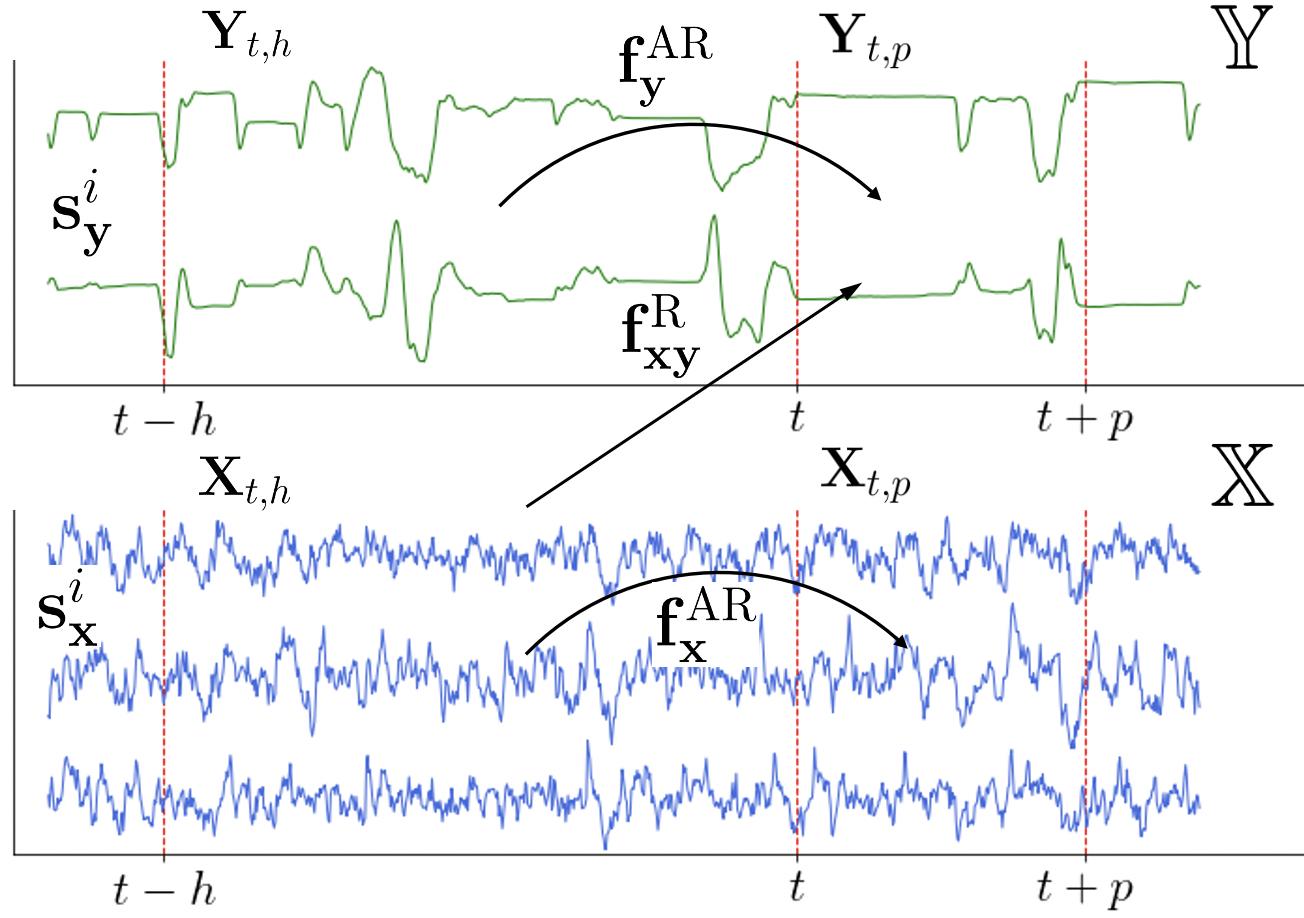
\includegraphics[width=0.55\linewidth]{figs/time_series_decoding}
	\end{figure}
	\vspace{-0.2cm}
	$\mathcal{S}_{\bx} = \{\bs_{\bx}^i\}_{i=1}^m$ -- множество временных рядов. \\
	$\bx_t = ([\bs_{\bx}^1]_t, \dots, [\bs_{\bx}^m]_t) \in \bbR^m$ -- временное представление. \\
	$\bX_{t,h} = [\bx_{t - h + 1}, \dots, \bx_{t}]^{\T} \in \bbR^{h \times m}$ -- представление предыстории. \\
	$\bX_{t,p} = [\bx_{t + 1}, \dots, \bx_{t + p}]^{\T} \in \bbR^{p \times m}$ -- представление горизонта \\ прогнозирования. \\
	$\mathbf{f}^{\text{AR}}_{\bx}: \bbR^{h \times m} \rightarrow \bbR^{p \times m}$ -- авторегрессионная модель. \\
	$\mathbf{f}^{\text{R}}_{\bx\by}: \bbR^{h \times m} \rightarrow \bbR^{p \times r}$ -- регрессионная модель. \\
	$\mathbf{f}_{\bx\by}: \bbR^{h_x \times m} \times \bbR^{h_y \times r} \rightarrow \bbR^{p \times r}$ -- модель декодирования модель.
\end{frame}
%--------------------------------------------------------------------------------
\begin{frame}{Восстановление зависимости в исходном и целевом пространствах}
	\vspace{-0.05cm}
	\begin{figure}
   		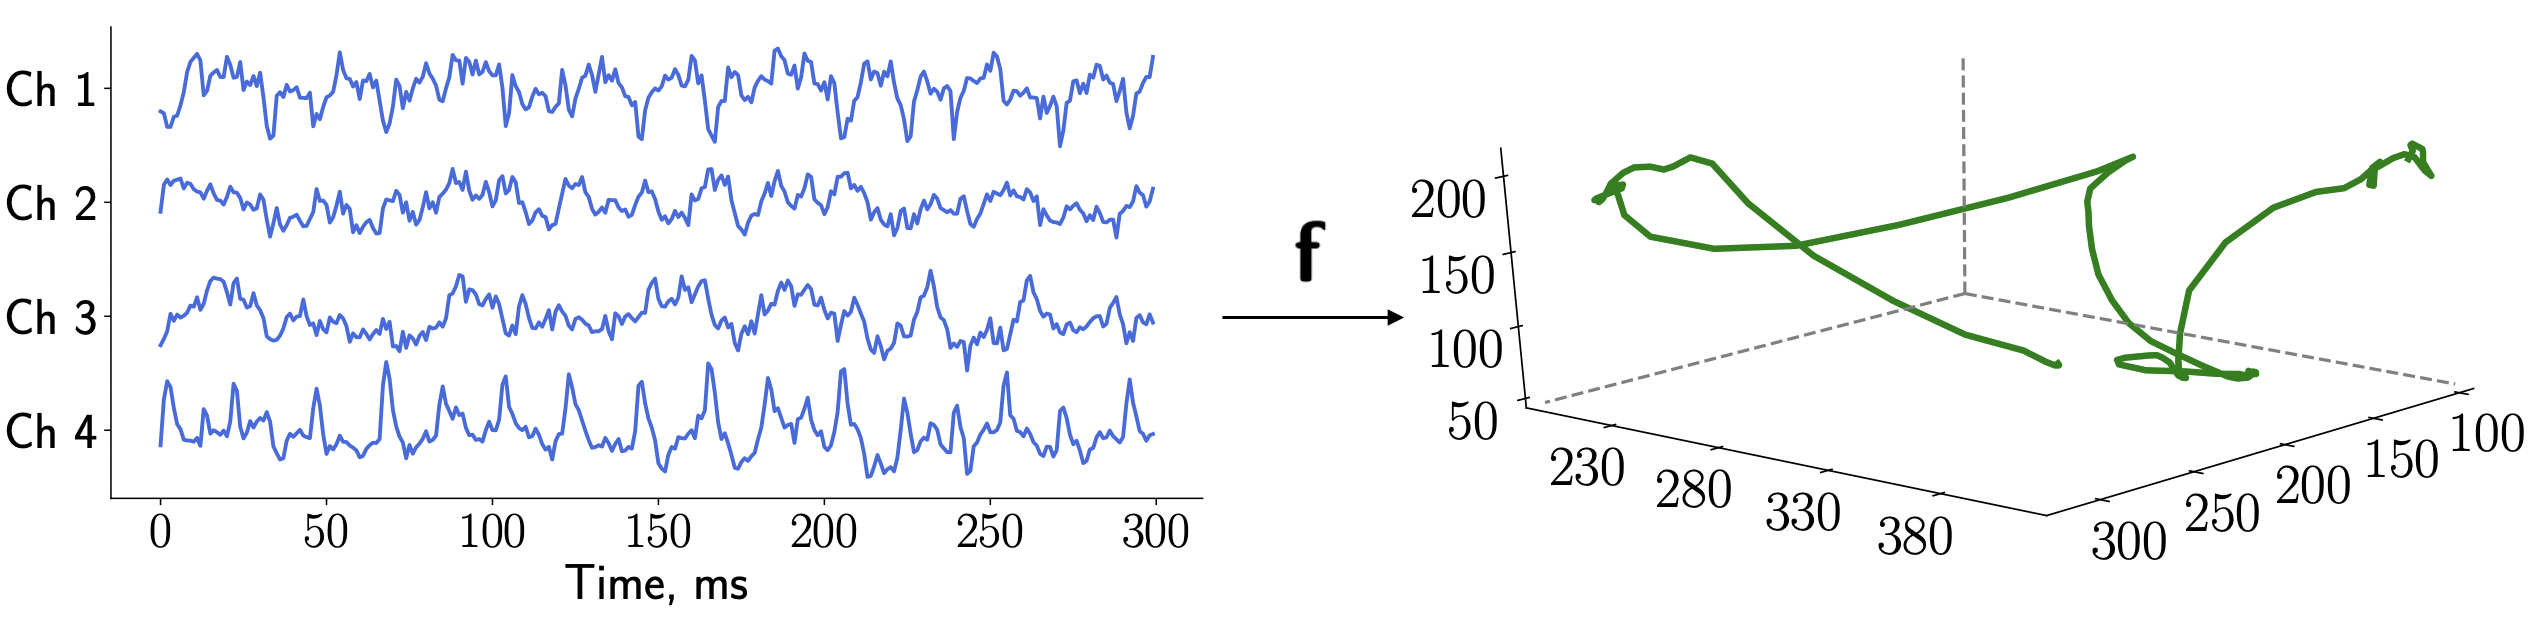
\includegraphics[width=\linewidth]{figs/slide3_1}
    \end{figure}
    \vspace{-0.15cm}
	\begin{minipage}{.48\linewidth}
		\vspace{-0.3cm}
		\begin{block}{Прогностическая модель декодирования}
			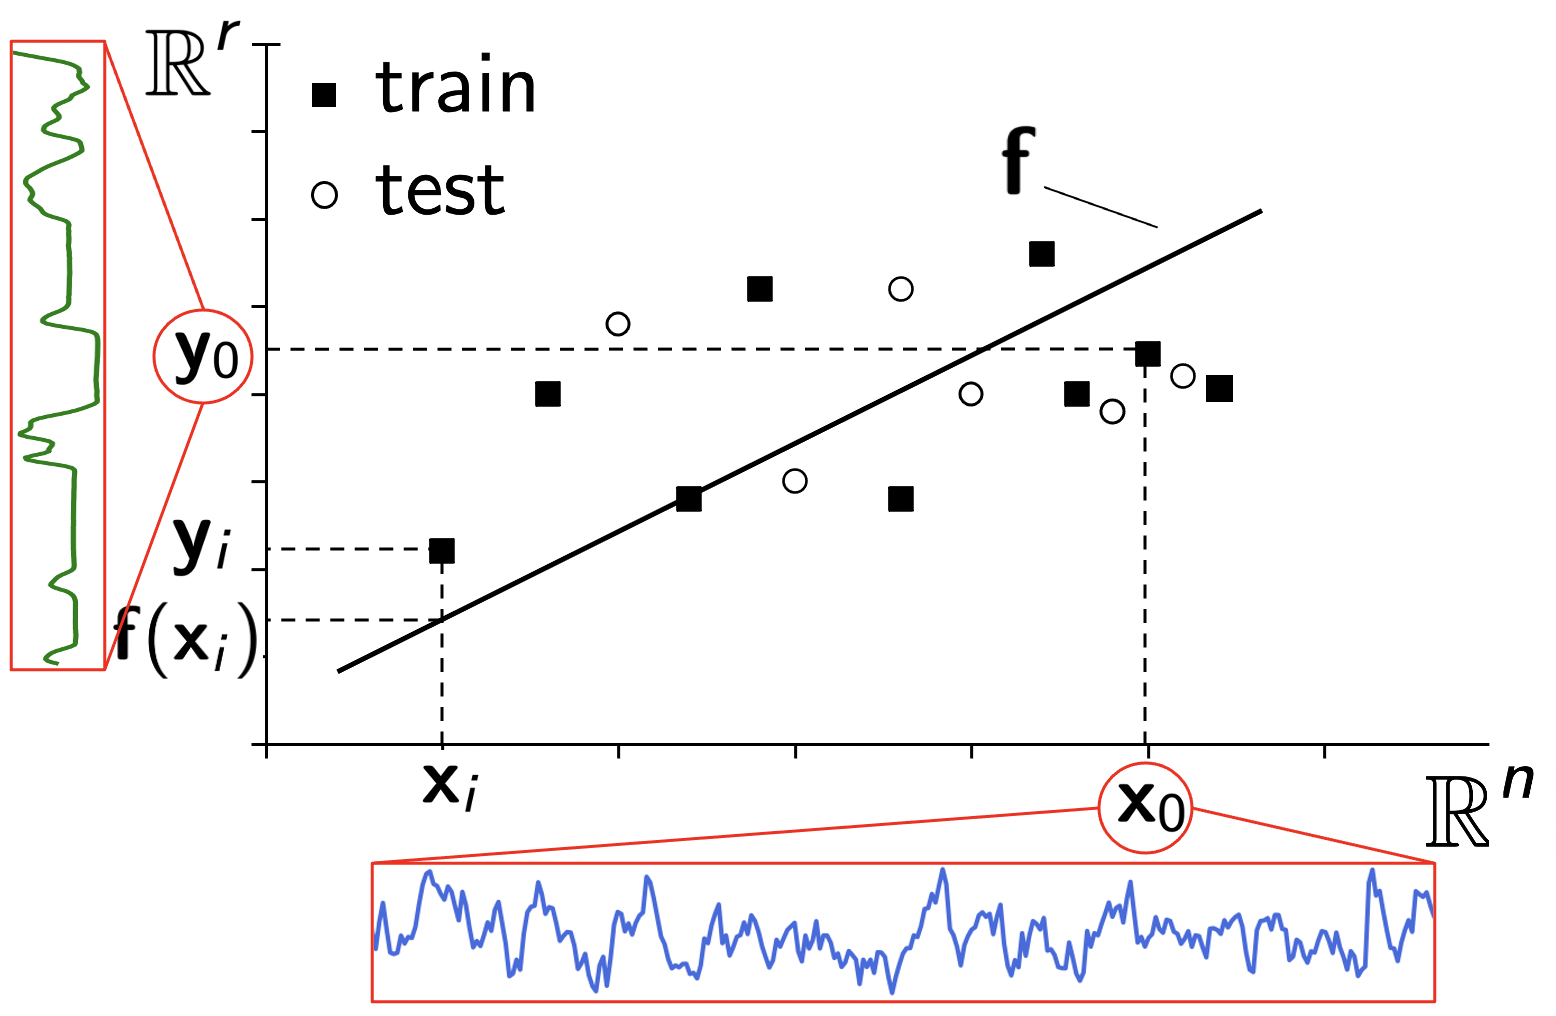
\includegraphics[width=\linewidth]{figs/slide3_3}
		\end{block}
	\end{minipage}%
	\begin{minipage}{.53\linewidth}
		\begin{block}{Согласование зависимостей в скрытом пространстве}
			\vspace{-0.7cm}
			\begin{equation*}
					\begin{tikzpicture}
						\matrix (m) [matrix of math nodes,row sep=2em,column sep=2em,minimum width=2em,ampersand replacement=\&]
						{
							\bx \in \bbR^n \& \& \by \in \bbR^r \\
							\& \bt, \bu \in \bbR^\ell \& \\};
						\path[-stealth]
						(m-1-1) edge node [above] {$\mathbf{f}$} (m-1-3)
						(m-1-1) edge [bend right=10] node [below, pos=0.3] {$\bW$} (m-2-2)
						(m-2-2) edge [bend right=10] node [above, pos=0.3] {$\bP$} (m-1-1)
						(m-1-3) edge [bend left=10] node [below, pos=0.3] {$\bC$} (m-2-2)
						(m-2-2) edge [bend left=10] node [above, pos=0.3] {$\bQ$} (m-1-3);
					\end{tikzpicture}
			\end{equation*}
			\vspace{-1.3cm}
			\begin{align*}
				\bx &= \bP \bt + \be_{\bx} \\
				\by &= \bQ \bu + \be_{\by} \\
			\end{align*}
			\vspace{-1.2cm}
			\[
				\text{cov} (\bt, \bu) \rightarrow \max_{\bP, \bQ}
			\]
		\end{block}
	\end{minipage}
\end{frame}
%--------------------------------------------------------------------------------
\begin{frame}{Задача декодирования сигналов}
	$\bY = \bF(\bX, \bTheta) + \bE_{\by} = \bX \cdot \bTheta^{\T}  + \bE_{\by}$ --  модель с параметрами $\bTheta \in \bbR^{r \times n}$.
	\begin{block}{Функция потерь модели декодирования}
		\vspace{-0.3cm}
		\[
			\mathcal{L}(f, \bX, \bY) = {\left\| \bY  - \bF(\bX, \bTheta) \right\| }_2^2 =  {\left\| \underset{m \times r}{\mathbf{Y}}  - \underset{m \times n}{\bX} \cdot \underset{r \times n}{\bTheta}^{\T} \right\| }_2^2 \rightarrow\min_{\bTheta}.
		\]
		\vspace{-0.3cm}
	\end{block}
	
	\begin{minipage}{0.65\linewidth}
		\begin{block}{Метод проекции в скрытое пространство}
		\vspace{-0.7cm}
		\begin{align*}
			\bX	&= \bT \bP^{\T} + \bE_{\bx},\\
			\bY &= \bU \bQ^{\T} + \bE_{\by}.
		\end{align*}
			\end{block}
	\end{minipage}%
	\begin{minipage}{0.35\linewidth}
			\vspace{-0.1cm}
			\begin{equation*}
				\begin{tikzpicture}
					\matrix (m) [matrix of math nodes,row sep=2em,column sep=4em,minimum width=2em,ampersand replacement=\&]
					{
						\bbX \subset \bbR^n \& \bbY \subset \bbR^r \\
						\bbT \subset \bbR^\ell \& \bbU \subset \bbR^s \\};
					\path[-stealth]
					(m-1-1) edge [black] node [black, above] {$\mathbf{f}$} (m-1-2)
					(m-1-1) edge [black, bend right=10] node [black, left] {$\bW$} (m-2-1)
					(m-2-1) edge [black, bend right=10] node [black, right] {$\bP$} (m-1-1)
					(m-1-2) edge [black, bend left=10] node [black, right] {$\bC$} (m-2-2)
					(m-2-2) edge [black, bend left=10] node [black, left] {$\bQ$} (m-1-2)
					(m-2-1) edge [black] node [black, above] {$\bB$} (m-2-2);
				\end{tikzpicture}
			\end{equation*}
	\end{minipage}
	\vspace{-0.4cm}
	\begin{block}{Согласование проекций}
		Для получения согласованной модели в скрытом пространстве находится функция связи 
		\vspace{-0.3cm}
		\[
			\bU = \bT \bB, \quad \bB = \text{diag}(\beta_k), \quad \beta_k = \bu_k^{\T}\bt_k / (\bt_k^{\T}\bt_k).
		\]
		Финальная модель декодирования имеет вид
		\vspace{-0.3cm}
		\[
			\bY = \bU \bQ^{\T} + \bE_{\by} \approx \bT \bB \bQ^{\T}+ \bE_{\by} = \bX \bW^* \bB \bQ^{\T} + \bE = \bX \bTheta^{\T} + \bE_{\by},
		\]
		\[
			\bT = \bX \bW^*, \quad \text{где \,} \bW^* = \bW (\bP^{\T} \bW)^{-1}.
		\]
	\end{block}
	 
\end{frame}
%--------------------------------------------------------------------------------
\begin{frame}{Согласование зависимостей в задаче декодирования}


	\textbf{Особенностью задачи} является избыточность размерности пространств переменных $\bx$ и $\by$.
	Требуется найти многообразия низкой размерности:
	\vspace{-0.2cm}
	\begin{equation*}
		\begin{tikzpicture}
			\matrix (m) [matrix of math nodes,row sep=2em,column sep=4em,minimum width=2em,ampersand replacement=\&]
			{
				\bbX \subset \bbR^n \& \bbY \subset \bbR^r \\
				\bbT \subset \bbR^\ell \& \bbU \subset \bbR^s \\};
			\path[-stealth]
			(m-1-1) edge [black] node [black, above] {$\mathbf{f}$} (m-1-2)
			(m-2-1) edge [black, bend right=10] node [black, right] {$\bphi_d$} (m-1-1)
			(m-2-2) edge [black, bend left=10] node [black, left] {$\bpsi_d$} (m-1-2)
			(m-1-1) edge [black, bend right=10] node [black, left] {$\bphi_e$} (m-2-1)
			(m-1-2) edge [black, bend left=10] node [black, right] {$\bpsi_e$} (m-2-2)
			(m-2-1) edge [black] node [black, above] {$\mathbf{h}$} (m-2-2);
		\end{tikzpicture}
	\end{equation*}
	$\bbT \subset \bbR^\ell$ и $\bbU \subset \bbR^s$ \textit{скрытые пространства} для $\bbX \in \bbR^n$ ($\ell \leq n$) и $\bbY \in \bbR^r (s \leq r)$, если существуют \textit{функции кодирования} $\bphi_e: \bbX \to \bbT$, $\bpsi_e: \bbY \to \bbU$ и \textit{декодирования} $\bphi_d: \bbT  \to \bbX$, $\bpsi_d: \bbU  \to \bbY$:
	\begin{align*}
	\text{для любого } \bx \in \bbX &\quad \text{существует } \bt \in \bbT: \bphi_d \bigl(\bphi_e(\bx)\bigr) = \bphi_d(\bt) = \bx; \\
	\text{для любого } \by \in \bbY &\quad  \text{существует } \bu \in \bbU: \bpsi_d \bigl(\bpsi_e(\by)\bigr) = \bpsi_d(\bu) = \by.
	\end{align*}

	Cкрытыe пространства $\bbT$ и $\bbU$ называются \textbf{согласованными}, если существует \textit{функция связи} $\mathbf{h}: \bbT \rightarrow \bbU$:
	\vspace{-0.3cm}
	\[
		\by = \mathbf{f}(\bx) = \bpsi_d\Bigl(\mathbf{h}\bigl(\bphi_e(\bx)\bigr)\Bigr).
	 \]
	 \vspace{-0.5cm}
	 \begin{block}{Функция согласования проекций}
	 	\vspace{-0.3cm}
	 	\[
	 		g: \bbT \times \bbU \rightarrow \bbR, \quad g(\bt, \bu) = g(\bphi_e(\bx), \bpsi_e(\by)) \rightarrow \max_{\bphi_e, \bpsi_e, \bh}
	 	\]
	 	\vspace{-0.3cm}
	 \end{block}

\end{frame}
%--------------------------------------------------------------------------------
\begin{frame}{Согласованная модель проекции в скрытое пространство}
	\begin{statement}[Исаченко, 2017]
		Вычисленные вектора $\bt_k$ и $\bu_k$ с помощью итеративной процедуры обновления:
		\vspace{-0.2cm}
		\begin{align*}
			\bt_k &:= \frac{\bX_k \bw_k}{\|\bw_k\|}, \quad  \bw_k := \bX_k^{\T} \bu_{k-1} / (\bu_{k-1}^{\T} \bu_{k-1}); \\ 
			\bu_k &:= \frac{\bY_k \bc_k}{\| \bc_k \|}, \quad \bc_k := \bY_k^{\T} \bt_k / (\bt_k^{\T} \bt_k).
		\end{align*}
		\vspace{-0.5cm} \\
		обладают максимальной ковариацией $\textnormal{cov}(\bt, \bu)$.
	\end{statement}

	\begin{rustheorem}[Исаченко, 2017]
		В случае линейных функций декодирования $\bphi_e (\bT) = \bT \bP^{\T}$, $\bpsi_e (\bU) = \bU \bQ^{\T}$ и функции согласования $g(\bt, \bu) = \textnormal{cov}(\bt, \bu)$ параметры
		\[
		\bTheta = \bW (\bP^{\T} \bW)^{-1} \bB \bQ^{\T}
		\]
		являются оптимальными для модели $\bF(\bX, \bTheta)$.
	\end{rustheorem}
\end{frame}
%--------------------------------------------------------------------------------
\begin{frame}{Согласованная модель проекции в скрытое пространство}
	\begin{block}{Principal Component Analysis}
		\vspace{-0.3cm}
		\[
			\bphi_{\bx}(\bX) =  \underset{m \times n}\bX \cdot \underset{n \times l}\bP^{\T}, \quad	\bpsi_{\bx}(\bT) =  \underset{m \times l}\bT \cdot \underset{l \times n}\bP, \quad \bP \bP^{\T} = \bI.
		\]
		\[
			\bp = \argmax_{\|\bp\|_{2} = 1} g(\btau) = \argmax_{\|\bp\|_{2} = 1} [\text{var}(\bX \textbf{p})],
		\]
		\vspace{-0.3cm}
	\end{block}
	\begin{block}{Partial Least Squares/Canonical Correlation Analysis}
		\vspace{-0.7cm}
		\begin{align*}
			\bphi_{\bx}(\bX) &= \bX \bW, \quad \bphi_{\by}(\bY) = \bY \bC, \\
			\bpsi_{\bx}(\bT) &= \bT \bP^{\T}, \quad \bpsi_{\by}(\bU) = \bU \bQ^{\T}.
		\end{align*}
		\[
			g(\btau, \bnu) = \text{cov}(\btau, \bnu), \quad g(\btau, \bnu) = \text{corr}(\btau, \bnu).
		\]
	\end{block}
	\begin{block}{Deep CCA}
		\vspace{-0.7cm}
		\begin{multline*}
			\max_{\|\bp\|_{2}=\|\bq\|_{2}=1}\left[ \text{corr}(\bphi_{\bx}(\bX) \cdot \bp, \bphi_{\by}(\bY) \cdot \bq)^{2}\right] = \\ = \max_{\bp, \bq} \frac{\bp^{\T} \bphi_{\bx}(\bX)^{\T} \bphi_{\by}(\bY) \bq}{\sqrt{\bp^{\T} \bphi_{\bx}(\bX)^{\T}  \bphi_{\bx}(\bX, \bW_{\bx}) \bp} \sqrt{\bq^{\T} \bphi_{\by}(\bY)^{\T}  \bphi_{\by}(\bY) \bq}}.
		\end{multline*}
	\end{block}
\end{frame}
%--------------------------------------------------------------------------------
\begin{frame}{Пример согласованной проекции в скрытое пространство}
	Исходные переменные $\bx_i \sim \mathcal{N}(0, \mathbf{\Sigma})$. \\ 
	Целевые переменные $\by_i$ линейно зависят от $pc_2$ и не зависят от $pc_1$.
	\begin{figure}[h]
	\centering
	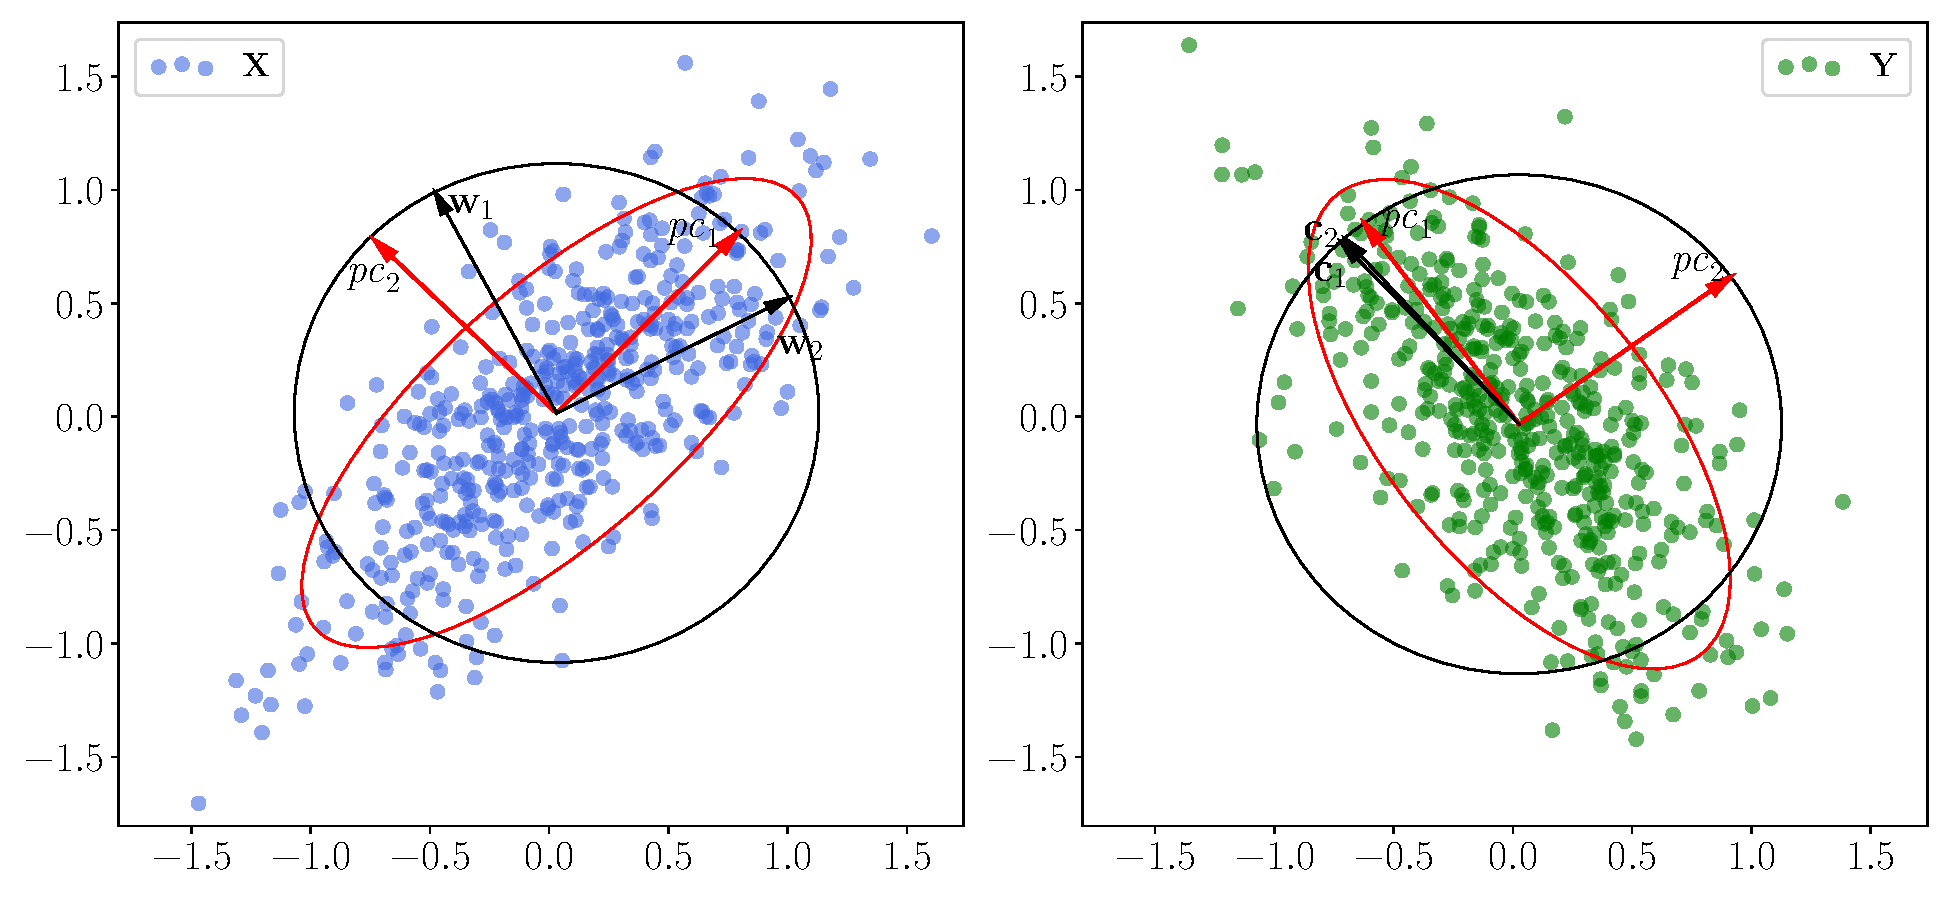
\includegraphics[width=0.8\linewidth]{figs/pls_toy_example}
	\end{figure}
	
	\begin{table}[]
		\centering
		\begin{tabular}{|l|c|c|c|c|}
			\hline
			& \textbf{LR} & \textbf{PCA}   & \textbf{PLS}  &  \textbf{CCA}  \\ \hline
			\textbf{MSE} & 0.01 &  0.24   &  0.13 &  0.13 \\ \hline
		\end{tabular}
	\end{table} 
	Согласование проекций матриц~$\bX$ и~$\bY$ находит оптимальное скрытое представление, отклоняя вектора~$\bw_k$ и~$\bc_k$ от направления главных компонент. 
\end{frame}
%--------------------------------------------------------------------------------
\begin{frame}{Суперпозиция моделей декодирования сигналов}
	Пусть $\mathbf{f}_1(\bx_1, \bTheta_1)$, $\mathbf{f}_2(\bx_2, \bTheta_2)$ -- линейные модели декодирования сигналов. 
	\begin{statement}[Исаченко, 2021]
		Пусть модель декодирования является аддитивной суперпозицией линейных моделей:
		\vspace{-0.3cm}
		\[
			\by = \mathbf{f}_1(\bx_1, \bTheta_1) + \mathbf{f}_2(\bx_2, \bTheta_2) + \boldsymbol{\varepsilon}_{\by} = \bTheta_1 \bx_1 + \bTheta_2 \bx_2 + \boldsymbol{\varepsilon}_{\by}.
		\]
		Тогда оптимальные параметры
		\vspace{-0.2cm}
		\begin{align*}
			\bTheta_1 &= (\bX_1^{\T} \bM_{\bX_2} \bX_1)^{-1} \bX_1^{\T} \bM_{\bX_2} \bY, \\
			\bTheta_2 &= (\bX_2^{\T} \bM_{\bX_1} \bX_2)^{-1} \bX_2^{\T} \bM_{\bX_1} \bY,
		\end{align*}
		где \, $\bM_{\bX_1} = \bI - \bX_1 (\bX_1^{\T} \bX_1)^{-1} \bX_1^{\T}$, \, $\bM_{\bX_2} = \bI -\bX_2 (\bX_2^{\T} \bX_2)^{-1} \bX_2^{\T}$.
	\end{statement}
	\begin{rustheorem}[Исаченко, 2021]
		Если $\text{span}(\bX_1) \neq \text{span}(\bX_2)$, то ошибка аддитивной суперпозиции линейных моделей декодирования не превышает ошибки отдельной модели:
		\begin{align*}
			\mathcal{L}_{\textnormal{sup}}(\bTheta_1^*, \bTheta_2^*, \bX_1, \bX_2, \bY) &\leq \mathcal{L}(\bTheta_1, \bX_1, \bY), \\
			\mathcal{L}_{\textnormal{sup}}(\bTheta_1^*, \bTheta_2^*, \bX_1, \bX_2, \bY) &\leq \mathcal{L}(\bTheta_2, \bX_2, \bY).
		\end{align*}
	\end{rustheorem}
\end{frame}
%--------------------------------------------------------------------------------
\begin{frame}{Суперпозиция моделей декодирования сигналов}
	Пусть $\mathbf{f}_1(\bx_1, \bTheta_1)$, $\mathbf{f}_2(\bx_2, \bTheta_2)$ -- линейные модели декодирования сигналов. 
	
	\begin{statement}[Исаченко, 2021]
		Пусть модель декодирования является аддитивной суперпозицией линейных моделей:
		\vspace{-0.3cm}
		\[
			\by = \mathbf{f}_1(\bx_1, \bTheta_1) + \mathbf{f}_2(\bx_2, \bTheta_2) + \boldsymbol{\varepsilon}_{\by} = \bTheta_1 \bx_1 + \bTheta_2 \bx_2 + \boldsymbol{\varepsilon}_{\by}.
		\]
		Оптимальная подматрица $\bTheta_2$ является решением задачи регрессии
		\[
			\| \bY_1 -  \bX_{21} \bTheta_2 \|^2 \rightarrow \min_{\bTheta_2},
		\]
		где $\bY_1 = \bM_{\bX_1} \bY$, $\bX_{21} = \bM_{\bX_1} \bX_2$.
	\end{statement}
	\begin{rustheorem}[Исаченко, 2021]
		Пусть  выполнены следующие условия
		\[
			\bY \neq \bP_{\bX_2} \bY, \quad \bX_1 \neq \bP_{\bX_2} \bX_1, \quad \bY^{\T} \bM_{\bX_2} \bX_1 \neq \bZero.
		\]
		Тогда выполнено строгое неравенство
		\[
			\cL_{\textnormal{sup}}(\bTheta_1^*, \bTheta_2^*, \bX_1, \bX_2, \bY) < \cL(\bTheta_2, \bX_2, \bY).
		\]
	\end{rustheorem}
\end{frame}
%--------------------------------------------------------------------------------
\begin{frame}{Нелинейные методы согласования скрытого пространства}
	Функции кодирования и декодирования являются глубокими нейросетями:
	\vspace{-0.1cm}
	\begin{align*}
		\bT &= \bphi_e(\bX) =  \bW_x^L \sigma(\dots \sigma(\bW_x^2 \sigma(\bX \bW_x^1)) \dots ) \\
		\bU &= \bpsi_e(\bY) =  \bW_y^L \sigma(\dots \sigma(\bW_y^2 \sigma(\bY \bW_y^1)) \dots ) \\
		\bX &= \bphi_d(\bT) =  \bW_t^L \sigma(\dots \sigma(\bW_x^2 \sigma(\bT \bW_t^1)) \dots ) \\
		\bY &= \bpsi_d(\bU) =  \bW_u^L \sigma(\dots \sigma(\bW_y^2 \sigma(\bU \bW_u^1)) \dots )
	\end{align*}
	\vspace{-0.4cm}
	\begin{block}{Согласование проекций}
		\vspace{-0.3cm}
		\[
			g(\bT, \bU) \rightarrow \max_{\bW}, \quad \bW = \{\bW_x^i, \bW_y^i, \bW_t^i, \bW_u^i\}_{i=1}^L.
		\]
	\end{block}	
	\vspace{-0.3cm}
		Градиент функции согласования $g(\bt, \bu) = \textnormal{corr}(\bt, \bu)$ имеет вид
		\[
			\frac{\partial g(\bt, \bu)}{\partial \bt} = \frac{1}{\ell - 1} \left(\bSigma_1^{-1/2} \bU \bV^{\T} \bSigma_2^{-1/2} \bU - \bSigma_1^{-1/2} \bU \bD \bV^{\T} \bSigma_1^{-1/2} \right),
		\]
		где $\bU, \bD, \bV = \textnormal{SVD}(\bSigma)$, \, $\bSigma = \bSigma_1^{-1/2} \bSigma_{12} \bSigma_2^{-1/2} $, \, $\bSigma_1 = \frac{1}{\ell - 1} \bT \bT^{\T}$, \, $\bSigma_2 = \frac{1}{\ell - 1} \bU \bU^{\T}$, \, $\bSigma_{12} = \frac{1}{\ell - 1} \bT \bU^{\T}$.
\end{frame}
%--------------------------------------------------------------------------------
\begin{frame}{Выбор признаков в задаче декодирования}
	$\bX = [\bchi_1, \dots, \bchi_n] \in \bbR^{m \times n}$~-- матрица исходных переменных; $\bY = [\bnu_1, \dots, \bnu_r] \in \bbR^{m \times r}$~-- матрица целевых переменных. \\
	Требуется найти бинарный вектор~$\ba = \{0, 1\}^n$, компоненты~-- индикаторы выбранных признаков. 
	\begin{block}{Функция ошибки отбора признаков}
		\vspace{-0.3cm}
		\[
			\bz = \argmin_{\bz' \in [0, 1]^n} S(\bz', \bX, \bY), \quad 
		a_j = [z_j > \tau].
		\]
		\vspace{-0.2cm}
	\end{block}
	\begin{block}{Функция ошибки модели декодирования}
		\vspace{-0.6cm}
		\[
			\mathcal{L}(\bTheta_{\ba}, \bX_{\ba}, \bY) = {\left\| \mathbf{Y} - \bX_{\ba}\bTheta^{\T}_{\ba} \right\| }_2^2 \rightarrow\min_{\bTheta_{\ba}}, \quad \bX_{\ba} = \{\bchi_j: a_j = 1, \, j = 1, \dots, n\}
		\]
		\vspace{-0.6cm}
	\end{block}
	\begin{block}{Задача квадратичного программирования}
	\vspace{-0.3cm}
	\[
	S(\bz, \bX, \bnu) = (1 - \alpha) \cdot \underbrace{\bz^{\T} \bQ \bz}_{\text{Sim}(\bX)} - \alpha \cdot \underbrace{\vphantom{()} \mathbf{b}^{\T} \bz}_{\text{Rel}(\bX, \bnu)} \rightarrow \min_{\substack{\bz \geq \bZero_n \\ \bOne_n^{\T} \bz=1}}.
	\]
	\vspace{-0.5cm}
	\end{block}
		$\bz \in [0, 1]^n$ -- значимость признаков; \\
		$\bQ = \bigl[\left|\text{corr}(\bchi_i, \bchi_j)\right|\bigr]_{i,j=1}^n \in \bbR^{n \times n}$ -- матрица парных взаимодействий признаков; \\
		$\mathbf{b} = \bigl[\left|\text{corr}(\bchi_i, \bnu)\right|\bigr]_{i=1}^n \in \bbR^n$ -- вектор релевантностей признаков к целевой переменной. 
\end{frame}
%--------------------------------------------------------------------------------
\begin{frame}{Выбор признаков с помощью квадратичного программирования}

	\begin{block}{Задача квадратичного программирования}
		\vspace{-0.3cm}
		\[
		S(\bz, \bX, \bnu) = (1 - \alpha) \cdot \underbrace{\bz^{\T} \bQ \bz}_{\text{Sim}(\bX)} - \alpha \cdot \underbrace{\vphantom{()} \mathbf{b}^{\T} \bz}_{\text{Rel}(\bX, \bnu)} \rightarrow \min_{\substack{\bz \geq \bZero_n \\ \bOne_n^{\T} \bz=1}}.
		\]
		\vspace{-0.5cm}
	\end{block}

	\begin{rustheorem}[Исаченко, 2018]
		Пусть матрица парных взаимодействий признаков $\hat{\bQ}$ получена полуопределенной релаксацией исходной матрицы $\bQ$:
		\vspace{-0.2cm}
		\begin{equation*}
			\hat{\bQ} = \bQ - \lambda_{\min}(\bQ) \bI.
		\end{equation*}
		\vspace{-0.7cm} \\
		Тогда задача выбора признаков с помощью квадратичного программирования имеет единственный глобальный минимум.
	\end{rustheorem}
	\begin{block}{Агрегирование релевантностей по целевым векторам (RelAgg)}
	\vspace{-0.2cm}
		\[
			\bb = \bigl[\left|\text{corr}(\bchi_i, \bnu)\right|\bigr]_{i=1}^n \rightarrow \bb = \left[\sum_{k=1}^r\left|\text{corr}(\bchi_i, \bnu_k)\right|\right]_{i=1}^n.
		\]
	\end{block}
	{\bf Недостаток:} нет учёта зависимостей в целевом пространстве матрицы~$\bY$. 
	
\end{frame}
%--------------------------------------------------------------------------------
\begin{frame}{Выбор признаков в задаче декодирования}
	\begin{block}{Симметричный учёт значимостей (SymImp)}
	Штрафуем коррелированные целевые вектора с помощью~$\text{Sim} (\bY)$:
	\[
	S(\bz, \bX, \bY) = \alpha_1 \cdot \underbrace{\bz_x^{\T} \bQ_x \bz_x}_{\text{Sim}(\bX)} - \alpha_2 \cdot \underbrace{\bz_x^{\T} \bB \bz_y}_{\text{Rel}(\bX, \bY)} + \alpha_3 \cdot \underbrace{\bz_y^{\T} \bQ_y \bz_y}_{\text{Sim}(\bY)} \rightarrow \min_{\substack{\bz_x \geq \bZero_n, \, \bOne_n^{\T}\bz_x=1 \\ \bz_y \geq \bZero_r, \, \bOne_r^{\T}\bz_y=1}},
	\]
	\[
	\bQ_x = \bigl[ \left| \text{corr}(\bchi_i, \bchi_j) \right| \bigr]_{i,j=1}^n, \,
	\bQ_y = \bigl[ \left| \text{corr}(\bnu_i, \bnu_j) \right| \bigr]_{i,j=1}^r, \,
	\bB =  \bigl[ \left| \text{corr}(\bchi_i, \bnu_j) \right| \bigr]_{\substack{i=1, \dots, n \\ j=1, \dots, r}},
	\]
	\[
	\alpha_1 + \alpha_2 + \alpha_3 = 1, \quad \alpha_i \geq 0.
	\] 
	\end{block}
	SymImp штрафует коррелированные целевые вектора, которые в меньшей мере объясняются признаками. 
		
	\begin{block}{Асимметричный учёт значимостей (AsymImp)}
		\vspace{-0.2cm}
		\begin{equation*}
		\alpha_1 \cdot \underbrace{\bz_x^{\T} \bQ_x \bz_x}_{\text{Sim}(\bX)} - \alpha_2 \cdot  \underbrace{\left(\bz_x^{\T} \bB \bz_y - \bb^{\T} \bz_y \right) }_{\text{Rel}(\bX, \bY)} + \alpha_3 \cdot \underbrace{\bz_y^{\T} \bQ_y \bz_y}_{\text{Sim}(\bY)} \rightarrow \min_{\substack{\bz_x \geq \bZero_n, \, \bOne_n^{\T}\bz_x=1 \\ \bz_y \geq \bZero_r, \, \bOne_r^{\T}\bz_y=1}}.
		\end{equation*}
		\vspace{-0.4cm} \\
		При $b_j = \max\limits_{i=1, \dots n} [\bB]_{i, j}$ коэффициенты при~$\bz_y$ в~$\text{Rel}(\bX, \bY)$ неотрицательны.
	\end{block}
\end{frame}
%--------------------------------------------------------------------------------
\begin{frame}{Выбор признаков в задаче декодирования}
	\[
		\alpha_1 \cdot \underbrace{\bz_x^{\T} \bQ_x \bz_x}_{\text{Sim}(\bX)} - \alpha_2 \cdot \underbrace{\vphantom{()} \bz_x^{\T}\mathbf{B} \bz_y}_{\text{Rel}(\bX, \bY)} \rightarrow \min_{\substack{\bz_x \geq \bZero_n \\ \bOne_n^{\T}\bz_x=1}}; \quad
		\alpha_3 \cdot \underbrace{\bz_y^{\T} \bQ_y \bz_y}_{\text{Sim}(\bY)} + \alpha_2 \cdot \underbrace{\vphantom{()} \bz_x^{\T} \mathbf{B} \bz_y}_{\text{Rel}(\bX, \bY)} \rightarrow \min_{\substack{\bz_y \geq \bZero_r  \\ \bOne_r^{\T}\bz_y=1}}.
	\]
	\vspace{-0.3cm}
	\begin{block}{Минимаксный подход (MinMax / MaxMin)}
		\vspace{-0.6cm}
		\[
		S(\bz, \bX, \bY) = \min_{\substack{\bz_x \geq \bZero_n \\ \bOne_n^{\T}\bz_x=1}} 	\max_{\substack{\bz_y \geq \bZero_r \\ \bOne_r^{\T}\bz_y=1}} \Bigl(\text {or} \, \max_{\substack{\bz_y \geq \bZero_r \\ \bOne_r^{\T}\bz_y=1}} \min_{\substack{\bz_x \geq \bZero_n \\ \bOne_n^{\T}\bz_x=1}}\Bigr) \Bigl[\alpha_1 \cdot \underbrace{\bz_x^{\T} \bQ_x \bz_x}_{\text{Sim}(\bX)} - \alpha_2 \cdot \underbrace{\bz_x^{\T} \bB \bz_y}_{\text{Rel}(\bX, \bY)} - \alpha_3 \cdot \underbrace{\bz_y^{\T} \bQ_y \bz_y}_{\text{Sim}(\bY)}\Bigr].
		\]
	\end{block}
	\vspace{-0.4cm}
	\begin{rustheorem}[Исаченко, 2018]
		Для положительно определенных матриц $\bQ_x$ и $\bQ_y$ minmax и maxmin задачи достигают одинакового значения функционала $S(\bz, \bX, \bY)$
	\end{rustheorem}
	\vspace{-0.2cm}
	\begin{rustheorem}[Исаченко, 2018]
		Минимаксная задача эквивалентна задаче квадратичного программирования с $n + r + 1$ переменными.
	\end{rustheorem}
	Для получения выпуклой задачи применяется полуопределенная рекласация сдвига спектра.

\end{frame}
%--------------------------------------------------------------------------------
\begin{frame}{Обобщение предложенных методов выбора признаков}
	\begin{rustheorem}[Исаченко, 2018]
		В одномерном случае $r=1$ предлагаемые методы выбора признаков SymImp, MinMax, MaxMin, AsymImp совпадают с исходной задачей минимизации функции ошибок $S(\bz, \bX, \bY)$.
	\end{rustheorem}
	\begin{table}
		\centering
		\footnotesize{
			\begin{tabular}{c|c|c}
				\hline
				Метод & Критерий & Функция ошибки $S(\bz, \bX, \bY)$ \\
				\hline && \\ 
				RelAgg & $\min \bigl[ \text{Sim}(\bX) - \text{Rel}(\bX, \bY) \bigr] $ & $\min\limits_{\bz_x} \bigl[ (1 - \alpha) \cdot \bz_x^{\T} \bQ_x \bz_x - \alpha \cdot \bz_x^{\T} \bB \bOne_r \bigr] $ \\ &&\\
				SymImp & $\begin{aligned} \min \, \bigl[ \text{Sim}(\bX) & - \text{Rel}(\bX, \bY) \\ & + \text{Sim}(\bY) \bigr] \end{aligned}$ & $ \min\limits_{\bz_x, \, \bz_y} \left[ \alpha_1 \cdot \bz_x^{\T} \bQ_x \bz_x - \alpha_2 \cdot \bz_x^{\T} \bB \bz_y + \alpha_3 \cdot \bz_y^{\T} \bQ_y \bz_y \right] $\\ &&\\ 
				MinMax & $\begin{aligned} &\min \, \bigl[ \text{Sim}(\bX) - \text{Rel}(\bX, \bY) \bigr]  \\ & \max \bigl[\text{Rel}(\bX, \bY) + \text{Sim}(\bY) \bigr] \end{aligned}$ & $	\min\limits_{\bz_x} 	\max\limits_{\bz_y} \bigl[\alpha_1 \cdot \bz_x^{\T} \bQ_x \bz_x - \alpha_2 \cdot \bz_x^{\T} \bB \bz_y - \alpha_3 \cdot \bz_y^{\T} \bQ_y \bz_y \bigr]$ \\ &&\\ 
				AsymImp & $\begin{aligned} & \min \, \bigl[ \text{Sim}(\bX) - \text{Rel}(\bX, \bY) \bigr]\\ &  \max \bigl[\text{Rel}(\bX, \bY) + \text{Sim}(\bY) \bigr] \end{aligned}$ & $\min\limits_{\bz_x, \bz_y} \bigl[ \alpha_1 \bz_x^{\T} \bQ_x \bz_x - \alpha_2 \left(\bz_x^{\T} \bB \bz_y - \bb^{\T} \bz_y \right) + \alpha_3  \bz_y^{\T} \bQ_y \bz_y \bigr]$\\  && \\
				\hline
		\end{tabular}}
	\end{table}
\end{frame}
%--------------------------------------------------------------------------------
\begin{frame}{Оптимизация нелинейных моделей с помощью квадратичного программирования}
	Метод Ньютона:
	\[
		\btheta^k = \btheta^{k - 1} + \Delta \btheta^{k - 1} = \btheta^{k-1} - \bH^{-1} \nabla S(\btheta).
	\]
	Обновление весов с выбором активных параметров:
	\begin{align*}
		\btheta_{\cA}^k &= \btheta_{\cA}^{k - 1} + \Delta \btheta_{\cA}^{k - 1}, \quad \btheta_{\cA} = \{\theta_j: j \in \cA \}, \\
		\btheta_{\bar{\cA}}^k &= \btheta_{\bar{\cA}}^{k - 1}, \quad \btheta_{\bar{\cA}} = \{\theta_j: j \notin \cA \}.
	\end{align*}
	Функция ошибки выбора активных параметров:
	\[
		\ba = \argmax_{\ba' \in \{1, 0\}^p} S(\ba', \bX, \by, \btheta) \Leftrightarrow \argmin_{\ba  \in \bbR^p_+, \, \|\ba\|_1=1} \bigl[\ba^{\T} \bQ \ba - \alpha \cdot \mathbf{b}^{\T} \ba \bigr].
	\]
	\vspace{-0.3cm}\\
	Параметр $\theta_j$ для модели $f(\bx, \btheta)$ является \textbf{активным}, если $\bJ^{\T} (\mathbf{f}(\bx, \btheta) - \by) \neq 0$. \\
	Функция ошибок для нелинейной регрессии:
	\vspace{-0.2cm}
	\[
		\cL(\btheta, \bX, \by) = \frac 12 \| \by - \mathbf{f}(\bX, \btheta) \|^2 = \frac 12 \sum_{i=1}^m \bigl( y_i - f(\bx_i,  \btheta)\bigr)^2,
	\]
	\vspace{-0.3cm}\\
	Функция ошибок для логистической регрессии:
	\vspace{-0.2cm}
	\[
		\cL(\btheta, \bX, \by) = \sum_{i=1}^m \bigl[y_i \log f (\bx_i , \btheta) + (1-y_i) \log \bigl(1 - f (\bx_i , \btheta)\bigr)\bigr].
	\]
\end{frame}
%--------------------------------------------------------------------------------
\begin{frame}{Оптимизация нелинейных моделей с помощью квадратичного программирования}
	\begin{rustheorem}[Исаченко, 2018]

		Пусть модель $f (\bx , \btheta)$ близка к линейной в окрестности точки $\btheta + \Delta \btheta$
		\[
			\mathbf{f}(\bX , \btheta + \Delta \btheta) \approx \mathbf{f}(\bX , \btheta) + \bJ \cdot \Delta  \btheta,
		\]
		где $\mathbf{J} \in \bbR^{m \times p}$ является матрицей Якоби.
		Тогда вектор обновления~$\Delta \btheta$ для функции ошибки нелинейной регрессии является решением задачи
		\[
			\| \be - \bF \Delta \btheta \|_2^2 \rightarrow \min_{\Delta \btheta \in \bbR^{p}}, \quad \be = \mathbf{f} - \by, \, \bF = \bJ.
		\]
	\end{rustheorem}
	\begin{rustheorem}[Исаченко, 2018]
		Пусть модель имеет вид $f(\bx , \btheta) = \sigma(\bx^{\T} \btheta)$. 
		Вектор обновлений $\Delta \btheta$ для функции ошибки логистической регрессии является решением задачи
		\[
			\| \be - \bF \Delta \btheta \|_2^2 \rightarrow \min_{\Delta \btheta \in \bbR^{p}}, \quad \be = \bR^{-1/2} (\by - \mathbf{f}), \, \bF = \bR^{1/2}\bX.
		\]
	\end{rustheorem}
\end{frame}
%--------------------------------------------------------------------------------
\begin{frame}{Оптимизация нелинейных моделей с помощью квадратичного программирования}
	\vspace{0.2cm}
	\begin{minipage}{.5\linewidth}
		\begin{figure}
			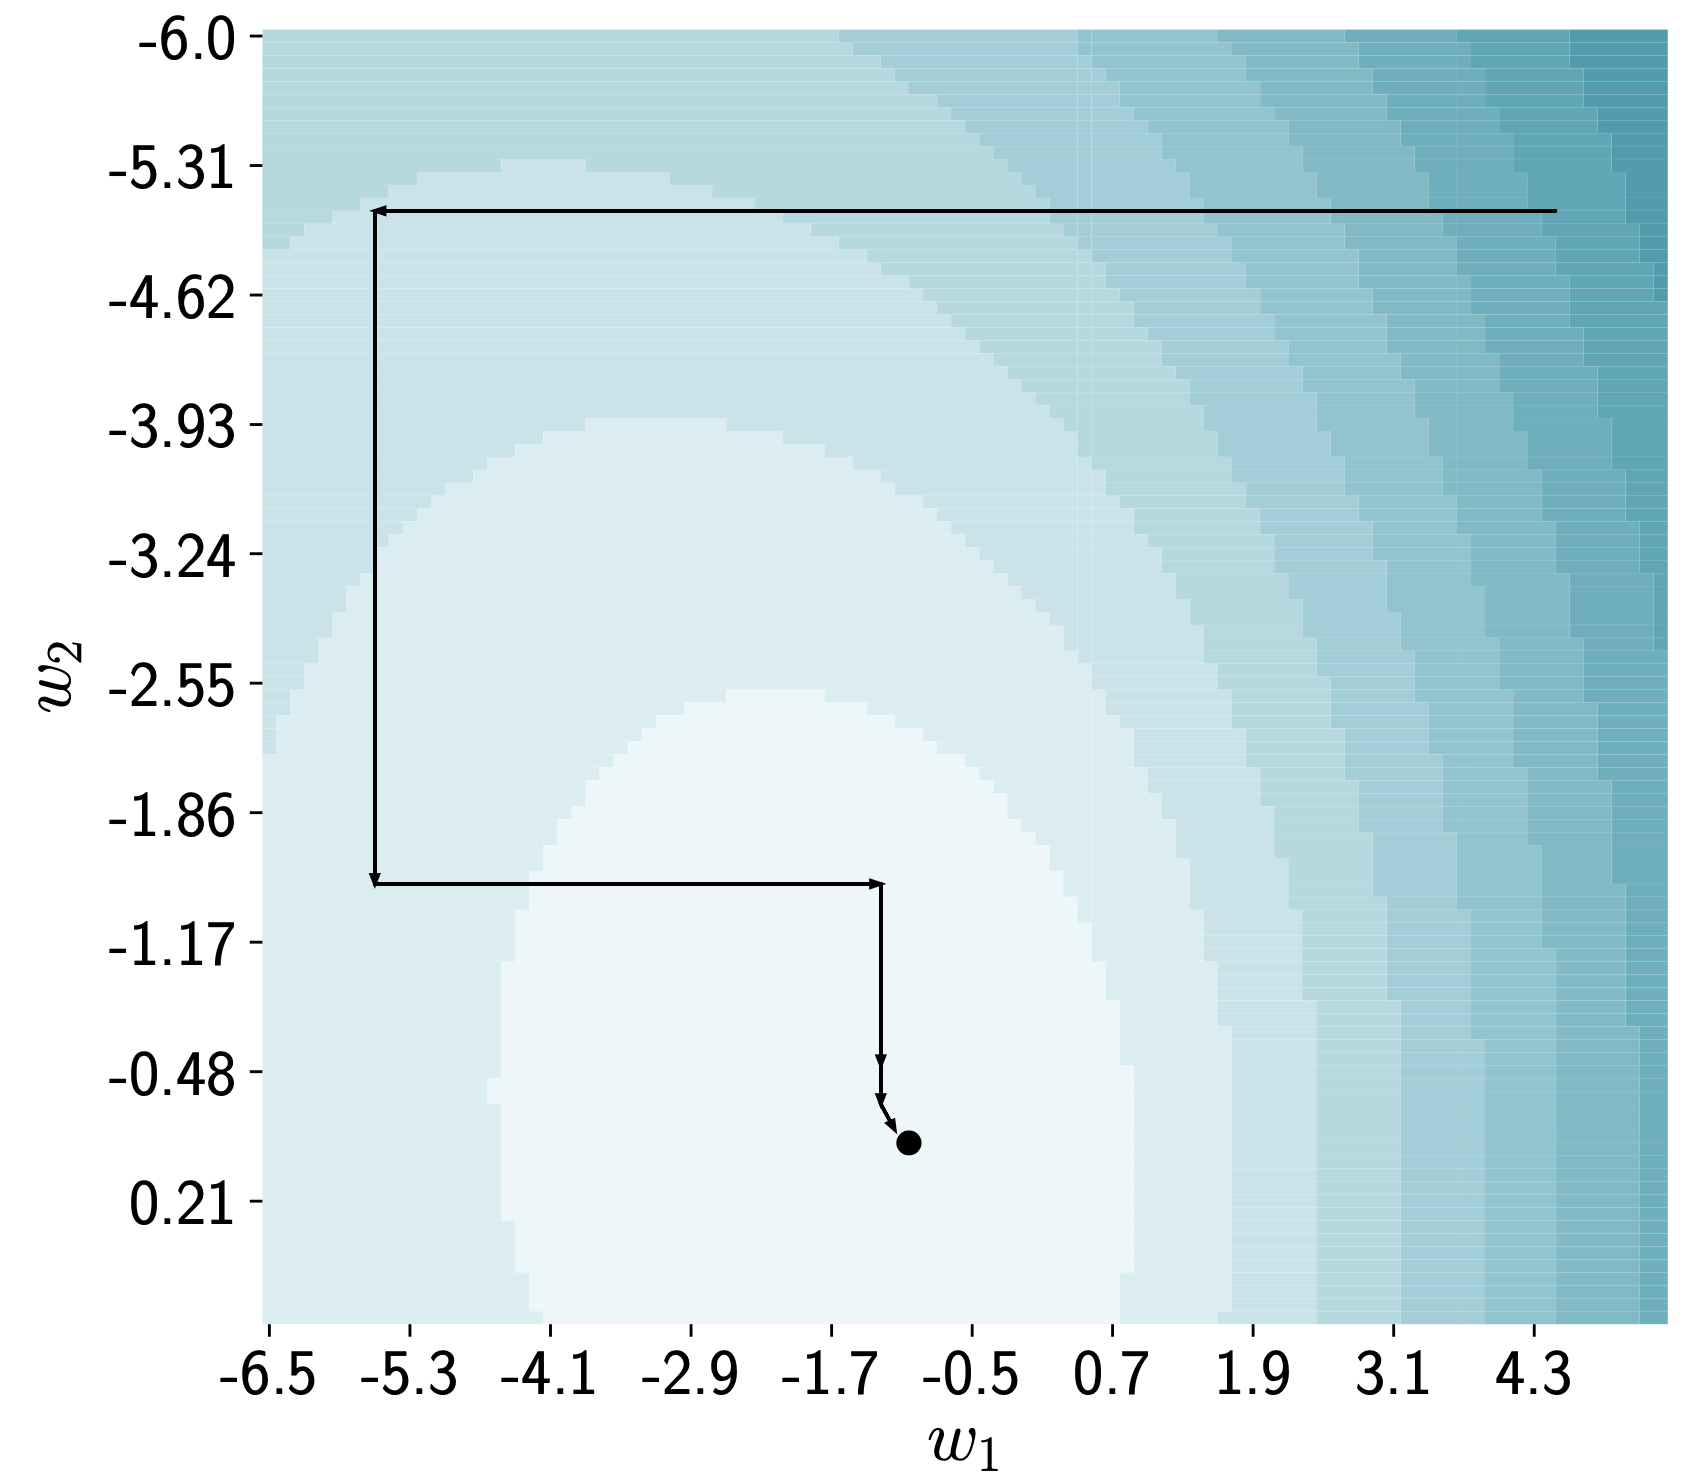
\includegraphics[width=0.8\linewidth]{figs/newton_qpfs}
		\end{figure}
	\end{minipage}%
	\begin{minipage}{.5\linewidth}
		\begin{figure}
			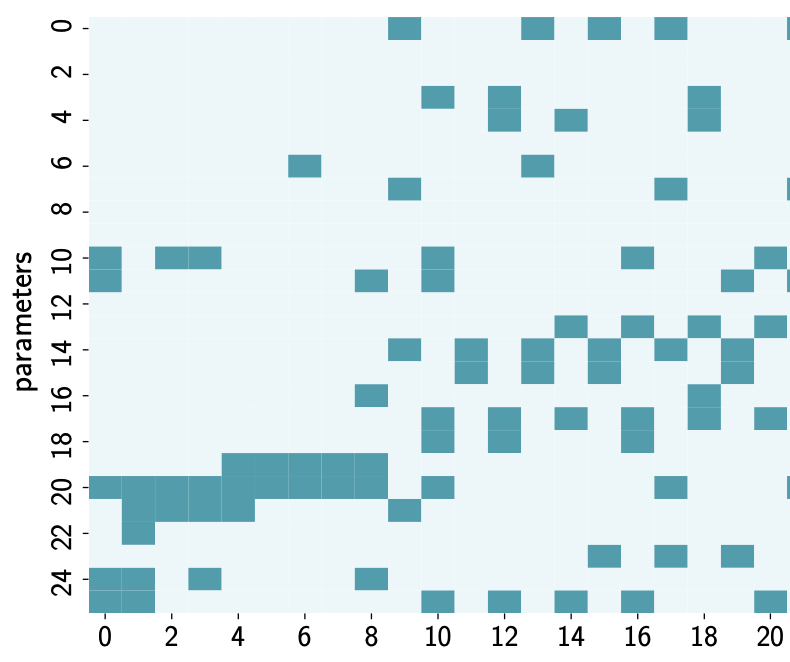
\includegraphics[width=0.8\linewidth]{figs/newton_params}
		\end{figure}
	\end{minipage}
	\begin{table}[h]
		\footnotesize
		\centering
		\begin{tabular}{|l|c|c|c|c|c|}
			\hline
			Выборка
			& GD 
			& Нестеров 
			& ADAM 
			& Ньютон 
			&
			\begin{tabular}[c]{@{}c@{}}QPFS+Ньютон\\ \end{tabular} \\ 
			\hline
			Boston House
			& $27.2\pm4.6$
			& $46.0\pm11.0$
			& $35.4\pm2.5$           
			& $22.1\pm15.2$            
			& $20.9\pm10.4$   \\  
			Prices
			& \multicolumn{1}{c|}{$32.4\pm5.6$}
			& \multicolumn{1}{c|}{$53.3\pm11.5$}
			& \multicolumn{1}{c|}{$37.8\pm7.0$}
			& \multicolumn{1}{c|}{$28.9\pm13.6$}
			& \multicolumn{1}{c|}{$\mathbf{24.5\pm9.4}$}\\ 
			\hline
			Communities
			& $48.0\pm6.4$
			& $31.4\pm2.8$
			& $23.3\pm3.7$        
			& $18.3\pm3.4$          
			&  $26.7\pm3.1$  \\ 
			and Crime
			& \multicolumn{1}{c|}{$47,5\pm6.5$}
			& \multicolumn{1}{c|}{$32.9\pm4.3$}
			& \multicolumn{1}{c|}{$28,1\pm4.5$}
			& \multicolumn{1}{c|}{$28.8\pm3.6$}
			& \multicolumn{1}{c|}{$\mathbf{28.4\pm3.0}$} \\ 
			\hline
			Forest
			& $18.9\pm0.4$
			& $1.83\pm0.4$
			& $1.81\pm0.6$             
			& $17.7\pm0.4$             
			& $17.9\pm0.4$   \\ 
			Fires
			& \multicolumn{1}{c|}{$\mathbf{20.0\pm2.1}$}
			& \multicolumn{1}{c|}{ $20.2\pm2.2$}
			& \multicolumn{1}{c|}{ $\mathbf{20.0\pm2.0}$}
			& \multicolumn{1}{c|}{ $20.6\pm1.4$}
			& \multicolumn{1}{c|}{ $20.2\pm2.2$} \\ 
			\hline
			Residential
			&  $51.6\pm17.7$
			&  $32.6\pm19.5$
			&  $30.0\pm24.8$            
			&  $35.5\pm24.7$            
			&   $30.3\pm10.7$ \\ 
			Building
			& \multicolumn{1}{c|}{ $53.7\pm13.9$}
			& \multicolumn{1}{c|}{ $34.1\pm13.6$}
			& \multicolumn{1}{c|}{ $34.1\pm19.4$}
			& \multicolumn{1}{c|}{ $35.0\pm15.6$}
			& \multicolumn{1}{c|}{ $\mathbf{30.9\pm5.3}$} \\ 
			\hline
		\end{tabular}
	\end{table}
\end{frame}
%--------------------------------------------------------------------------------
\begin{frame}{Внешние критерии качества решения задачи декодирования}

\begin{block}{Нормированное RMSE}
	Качество прогнозирования:
	\vspace{-0.2cm}
	\[
		\text{sRMSE}(\bY, \widehat{\bY}_{\ba}) = \sqrt{\frac{\text{MSE} (\bY, \widehat{\bY}_{\ba})}{\text{MSE} (\bY, \overline{\bY})}} =  \frac{\| \bY - \widehat{\bY}_{\ba} \|_2}{\| \bY - \overline{\bY} \|_2}, \quad \text{где} \quad \widehat{\bY}_{\ba} = \bX_{\ba} \bTheta_{\ba}^{\T}.
	\]
	\vspace{-0.2cm}
	$\overline{\bY}$~--- константный прогноз.
\end{block}

\begin{block}{Мультикорреляция}
	Среднее значение коэффициента множественной корреляции:
	\vspace{-0.2cm}
	\[
		R^2 = \frac{1}{r} \text{tr} \left( \bC^{\T} \mathbf{R}^{-1} \bC \right), \quad \bC = [ \text{corr}(\bchi_i, \bnu_j)]_{\substack{i=1, \dots, n \\ j=1, \dots, r}}, \, \mathbf{R} = [ \text{corr}(\bchi_i, \bchi_j)]_{i, j = 1}^n.
	\]
\end{block}
\vspace{-0.4cm}
\begin{block}{Байесовский информационный критерий}
	Компромисс между качеством предсказания и числом выбранных признаков~$\|\ba\|_0$:
	\vspace{-0.3cm}
	\[
		\text{BIC} = m \ln \left( \text{MSE} ( \bY, \widehat{\bY}_{\ba})\right) + \| \ba \|_0 \cdot \log m.
	\]
\end{block}
\end{frame}
%--------------------------------------------------------------------------------
\begin{frame}{Задача декодирования сигналов электрокортикограммы}
    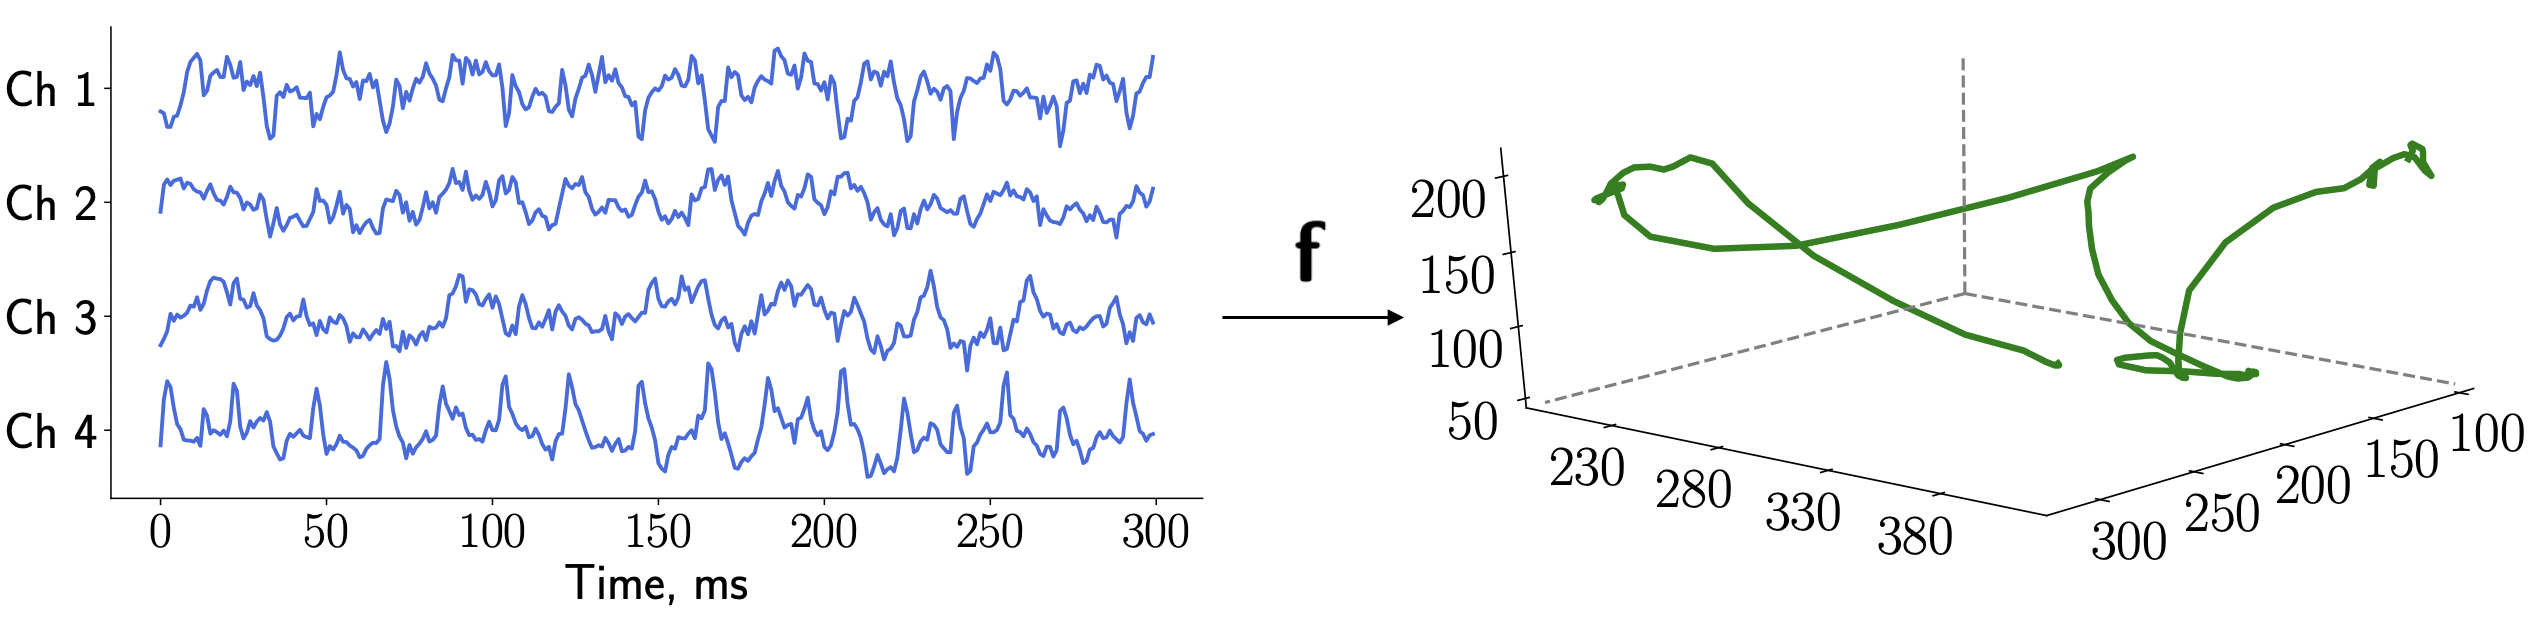
\includegraphics[width=1.0\linewidth]{figs/slide3_1}
	\begin{minipage}{.58\linewidth}
 	Заданы: \\
	$\bX \in \bbR^{m \times (32 \cdot 27)}$ -- сигналы ECoG, \\
	$\bY \in \bbR^{m \times 3k}$ -- траектория движения руки, где
	\vspace{0.1cm}
	\[
		\bY = 
		\begin{pmatrix}
		x_1 \,\, y_1 \,\, z_1 & \dots & x_{k\hphantom{+1}} \,\, y_{k\hphantom{+1}} \,\, z_{k\hphantom{+1}}\\
		x_2 \,\, y_2 \,\, z_2 & \dots & x_{k + 1} \,\, y_{k + 1} \,\, z_{k + 1}\\
		 \dots & \dots & \dots  \\
		x_m \, y_m \, z_m & \dots & x_{m + k} \, y_{m + k} \, z_{m + k}
		\end{pmatrix}.
	\]
	Столбцы матрицы $\bY$ сильно скоррелированы по временной оси.
	\end{minipage}%
	\begin{minipage}{.42\linewidth}
		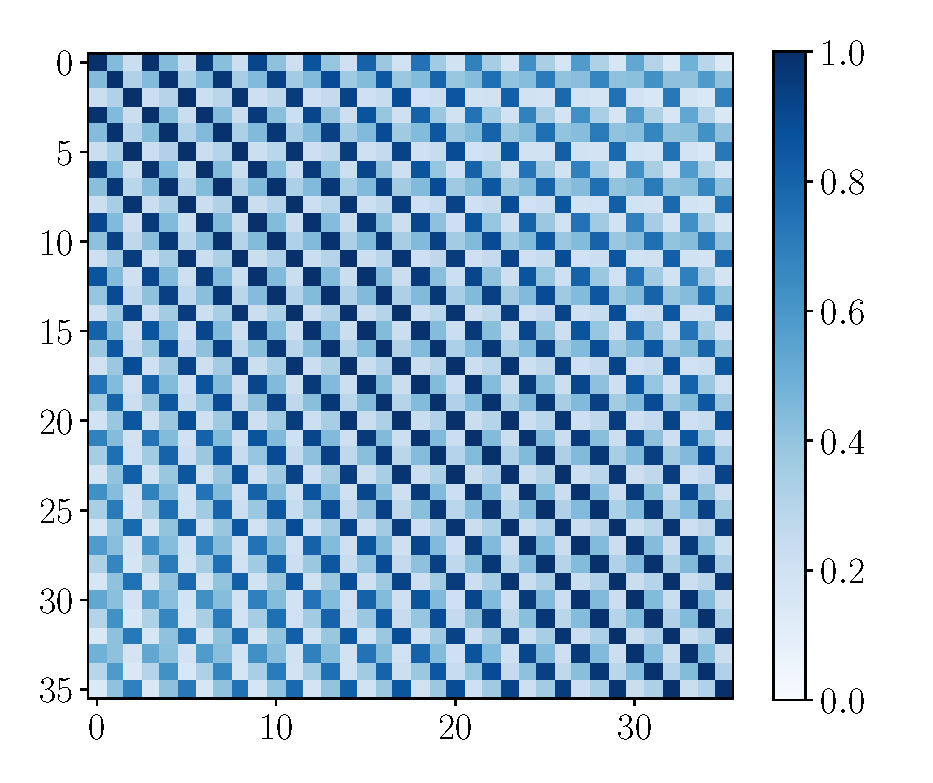
\includegraphics[width=\linewidth]{figs/Y_corr_matrix.eps} \\
		\centering Матрица корреляций $\bY$
	\end{minipage}
	\\
	\url{http://neurotycho.org}
\end{frame}
%--------------------------------------------------------------------------------
\begin{frame}{Анализ предложенных методов выбора признаков}
	\begin{figure}
		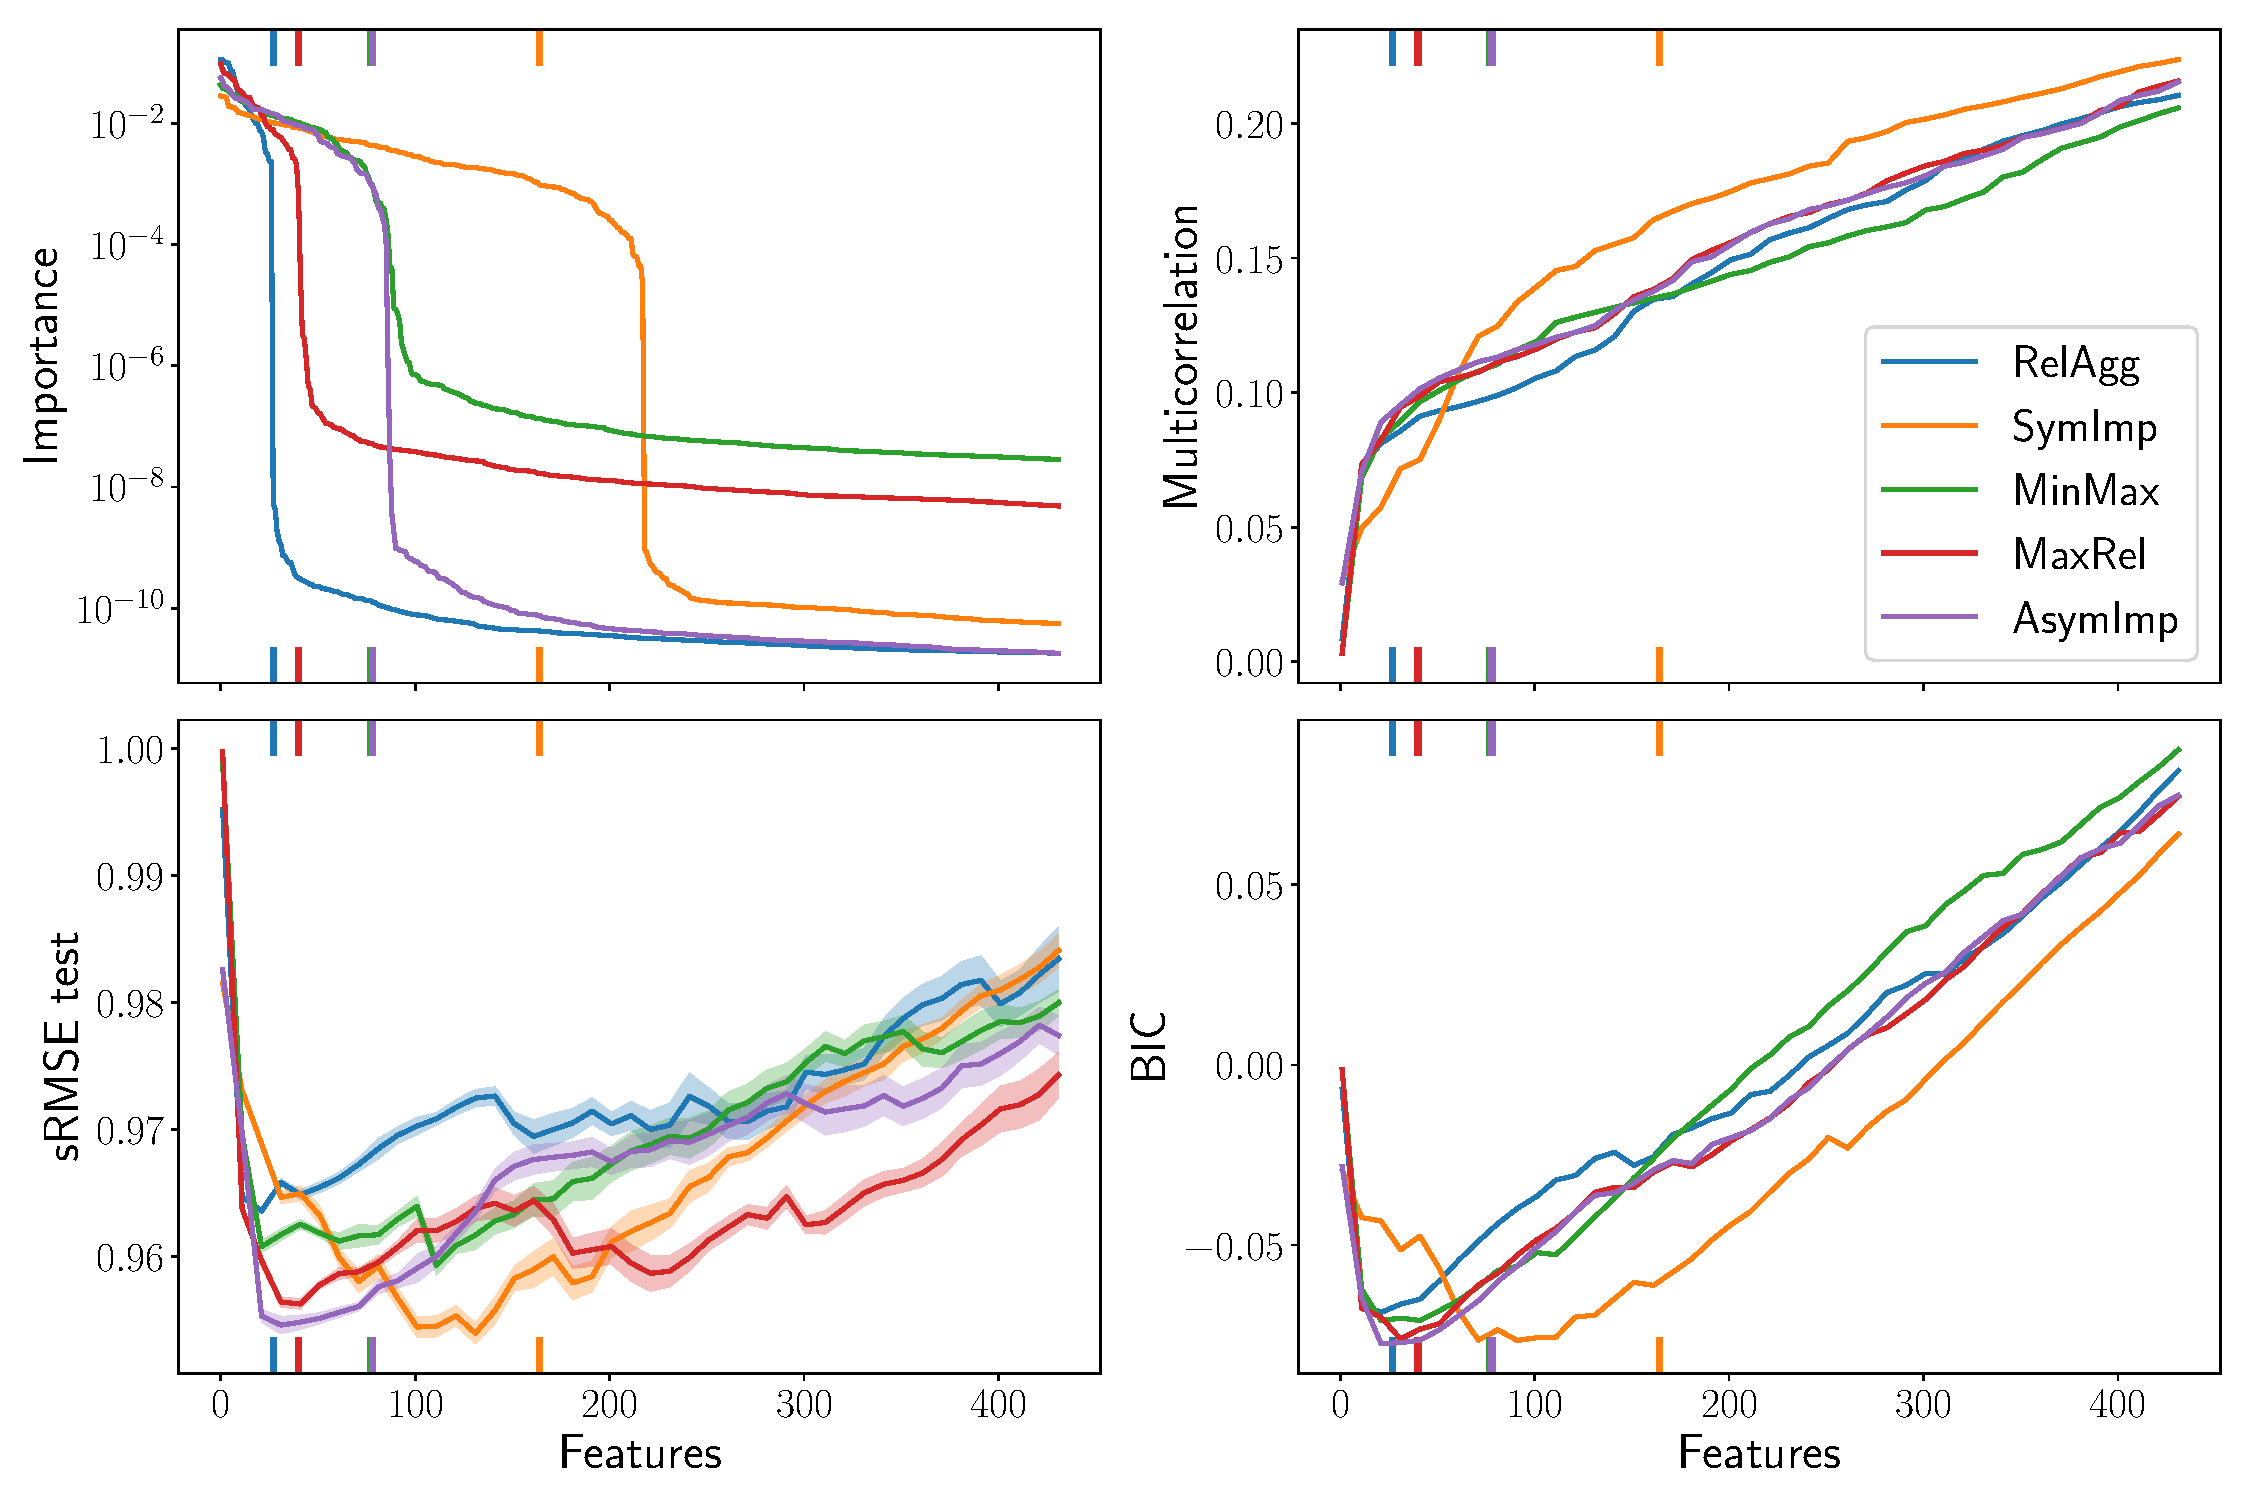
\includegraphics[width=0.9\linewidth]{figs/ecog_3_30_metrics.pdf}
		\vspace{-0.2cm}
	\end{figure}
	Предложены методы выбора модели, имеющей меньшую ошибкой по отношению к базовому алгоритму.
\end{frame}
%--------------------------------------------------------------------------------
\begin{frame}{Сравнение метода проекции в скрытое пространство с методами выбора признаков}

\begin{figure}[h]
	\begin{minipage}{.43\linewidth}
		\centering
		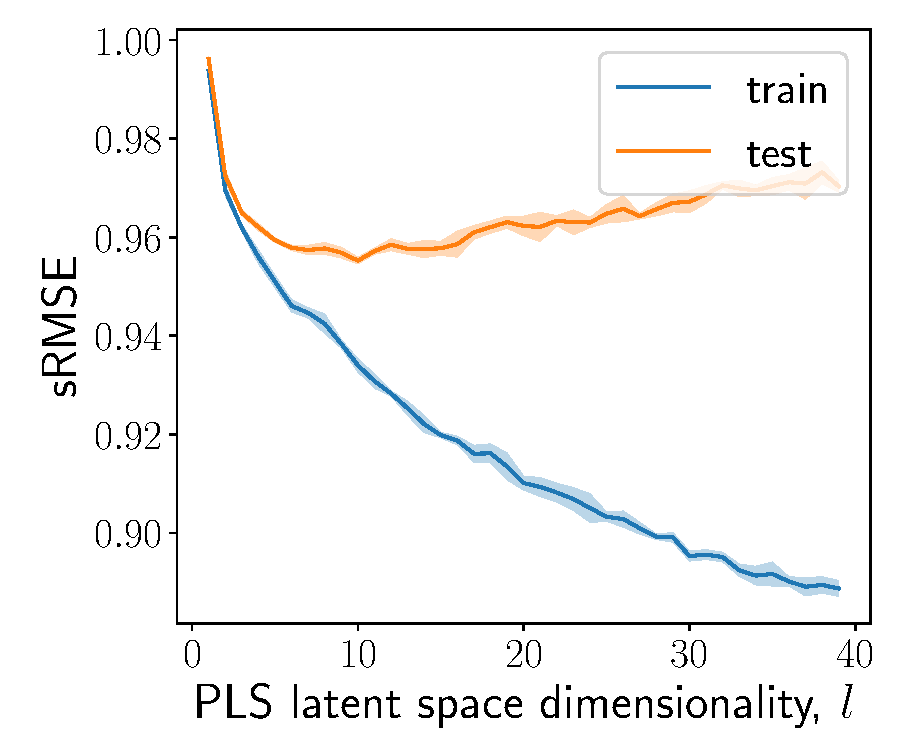
\includegraphics[width=1.\linewidth]{figs/pls_vs_k}
	\end{minipage}%
	\begin{minipage}{.57\linewidth}
		\centering
		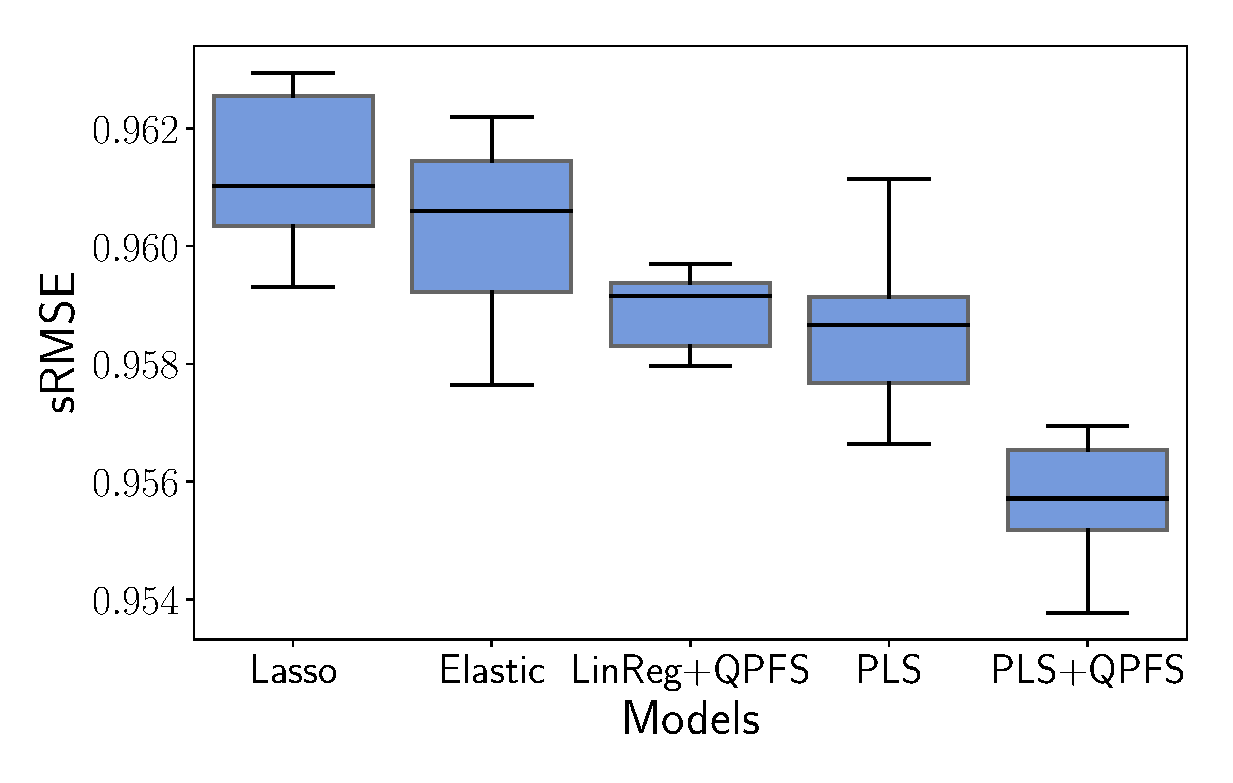
\includegraphics[width=1.\linewidth]{figs/models2}
	\end{minipage}
\end{figure}

\begin{table}[!h]
	\centering
	\begin{tabular}{l|ccccc}
		\hline
		& sRMSE  & $\|\ba\|_0$ & Spearman $\rho$ & $\ell_2$ \\ \hline
		RelAgg & 0.965 $\pm$ 0.002 & 26.8 $\pm$ 3.8 & 0.915 $\pm$ 0.016 & 0.145 $\pm$ 0.018   \\
		SymImp & 0.961 $\pm$ 0.001 & 224.4 $\pm$ 9.0 & 0.910 $\pm$ 0.017 & 0.025 $\pm$ 0.002   \\
		MinMax & 0.961 $\pm$ 0.002 & 101.0 $\pm$ 2.1& 0.932 $\pm$ 0.009 & 0.059 $\pm$ 0.004   \\
		AsymImp & 0.955 $\pm$ 0.001 & 85.8 $\pm$ 10.2& 0.926 $\pm$ 0.011 & 0.078 $\pm$ 0.007  \\ \hline
	\end{tabular}
	\label{ch3:tbl:stability}
\end{table}

\end{frame}
%--------------------------------------------------------------------------------
\begin{frame}{Пример прогноза движения руки по сигналам ECoG}
	\begin{figure}
		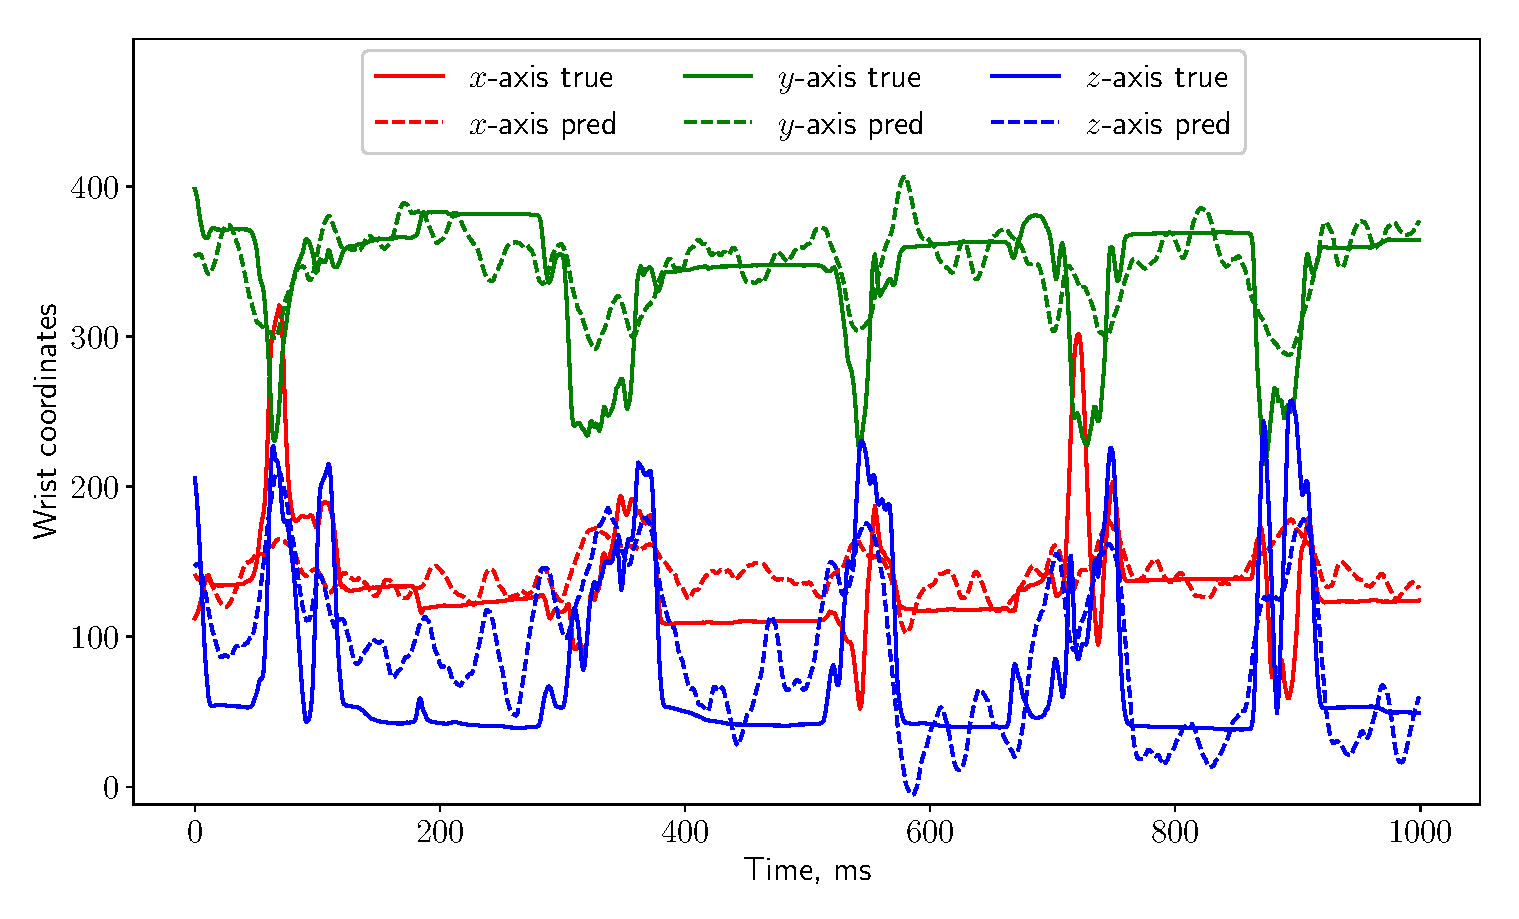
\includegraphics[width=0.9\linewidth]{figs/ecog_prediction}
	\end{figure}
\end{frame}
%--------------------------------------------------------------------------------
\begin{frame}{Результаты, выносимые на защиту}
\begin{enumerate}
	\item Исследована проблема снижения размерности сигналов в коррелированных пространствах высокой размерности. 
	Предложены методы декодирования сигналов, учитывающие зависимости как в исходном, так и в целевом пространстве сигналов.
	\vfill
	\item Доказаны теоремы об оптимальности предлагаемых методов декодирования сигналов. Предлагаемые методы выбирают согласованные модели в случае избыточной размерности описания данных.
	\vfill 
	\item Предложены методы выбора признаков, учитывающие зависимости как в исходном, так и в целевом пространстве. Предложенные методы доставляют устойчивые и адекватные решения в пространствах высокой размерности.
	\vfill
	\item Предложены нелинейные методы согласования скрытых пространств для данных со сложноорганизованной целевой переменной.
	\vfill
	\item Предложен ряд моделей для прогнозирования гетерогенных наборов сигналов для задачи построения нейрокомпьютерных интерфейсов.
\end{enumerate}
\end{frame}
%--------------------------------------------------------------------------------
\begin{frame}{Список работ автора по теме диссертации}
	\vspace{-0.1cm}
	\begin{block}{Публикации ВАК}
		\vspace{-0.1cm}
		{\scriptsize
		\begin{enumerate}
			\item Isachenko R., Strijov V. Quadratic Programming Feature Selection for Multicorrelated Signal Decoding with Partial Least Squares \emph{Expert Systems with Applications}, 2021, на рецензировании.
			\item Исаченко Р.В., Яушев Ф.Р., Стрижов В.В. Модели согласования скрытого пространства в задаче прогнозирования // Системы и средства информатики, 31(1), 2021.
			\item Isachenko~R., Vladimirova~M., Strijov~V. Dimensionality Reduction for Time Series Decoding and Forecasting Problems. \emph{DEStech Transactions on Computer Science and Engineering}, optim, 2018.
			\item Isachenko~R., Strijov~V. Quadratic programming optimization for Newton method. \emph{Lobachevskii Journal of Mathematics}, 39(9), 2018.
			\item Isachenko~R. et al. Feature Generation for Physical Activity Classification. \emph{Artificial Intellegence and Decision Making}, 3, 2018.
			\item Исаченко Р.В., Стрижов В. В. Метрическое обучение в задачах мультиклассовой классификации временных рядов \emph{Информатика и её применения}, 10(2), 2016.
		\end{enumerate}
	}
	\end{block}
\vspace{-0.3cm}
\begin{block}{Выступления с докладом}
	\vspace{-0.1cm}
	{\scriptsize
	\begin{enumerate}
		\item  Intelligent Data Processing Conference, 2020, Снижение размерности в задаче декодирования временных рядов.
		\item  Intelligent Data Processing Conference, 2018, Dimensionality reduction for multicorrelated signal decoding with projections to latent space. 
		\item Математические методы распознавания образов, 2017. Локальные модели для классификации объектов сложной структуры.
		\item Intelligent Data Processing Conference, 2016. Multimodel forecasting multiscale time series in internet of things.
		\item Ломоносов, 2016. Метрическое обучение в задачах мультиклассовой классификации временных рядов.
	\end{enumerate}
	}
\end{block}
\end{frame}
\end{document} 
